\documentclass[conference]{IEEEtran}
\IEEEoverridecommandlockouts
% The preceding line is only needed to identify funding in the first footnote. If that is unneeded, please comment it out.
\usepackage{cite}
\usepackage{amsmath,amssymb,amsfonts}
\usepackage{algorithmic}
\usepackage{graphicx}
\usepackage[inline]{enumitem} 
\usepackage{textcomp}
\usepackage[]{algorithm2e}
\usepackage{xcolor}
\usepackage[hyphens,spaces,obeyspaces]{url}
\usepackage{multirow}
\definecolor{LightGray}{gray}{0.9}
%%personal macros --begin%%
%%%%%%%%Useful macros for poof-reading, always copy-paste into your latex projects
\usepackage[colorinlistoftodos,prependcaption,textsize=tiny]{todonotes}
\usepackage{listings}
\usepackage{minted}

\newboolean{showcomments}
\setboolean{showcomments}{true} % toggle to show or hide comments
\ifthenelse{\boolean{showcomments}}
{\newcommand{\nb}[2]{
		\fcolorbox{black}{yellow}{\bfseries\sffamily\scriptsize#1}
		{\sf\small$\blacktriangleright$\textit{#2}$\blacktriangleleft$}
	}
	\newcommand{\version}{\emph{\scriptsize$-$working$-$}}
}
{\newcommand{\nb}[2]{}
	\newcommand{\version}{}
}
\newcommand\patrizio[1]{\nb{Patrizio}{#1}}
\newcommand\sergio[1]{\nb{Sergio}{#1}}
\newcommand\tb[1]{\nb{Thorsten}{#1}}

% Macros for proof-reading
\usepackage[normalem]{ulem} % for \sout
\usepackage{xcolor}
\usepackage{array}
\usepackage{booktabs}
\usepackage{scalerel}
\usepackage[para,online,flushleft]{threeparttable}
\usepackage{booktabs}
\usepackage{pifont}
\newcommand*\rot{\rotatebox{90}}
\newcommand*\OK{\ding{51}}
\newcommand{\xmark}{\ding{55}}%
\newcolumntype{P}[1]{>{\centering\arraybackslash}p{#1}}
\newcommand{\ra}{$\rightarrow$}
\newcommand{\ugh}[1]{\textcolor{red}{\uwave{#1}}} % please rephrase
\newcommand{\ins}[1]{\textcolor{blue}{\uline{#1}}} % please insert
\newcommand{\del}[1]{\textcolor{red}{\sout{#1}}} % please delete
\newcommand{\chg}[2]{\textcolor{red}{\sout{#1}}{\ra}\textcolor{blue}{\uline{#2}}} % please change
%%%%%%%%
%Macros
% Footnotes
\newcommand{\foot}[1]{\footnote{\url{#1}}}
%%personal macros --end%%
\def\BibTeX{{\rm B\kern-.05em{\sc i\kern-.025em b}\kern-.08em
    T\kern-.1667em\lower.7ex\hbox{E}\kern-.125emX}}

\begin{document}

\title{MoTiVML: A Variability Modelling Language for Flexible and Customizable Robotic System Design\\
%{\footnotesize \textsuperscript{*}Note: Sub-titles are not captured in Xplore and
%should not be used}
%\thanks{Identify applicable funding agency here. If none, delete this.}
}

\author{\IEEEauthorblockN{Jude Gyimah}
\IEEEauthorblockA{\textit{Department of Computer Science and Engineering} \\
\textit{Chalmers $|$ University of Gothenburg}\\
Gothenburg, Sweden \\
gusgyiju@student.gu.se}
\and
\IEEEauthorblockN{Sergio Garc\'{i}a}
\IEEEauthorblockA{\textit{Department of Computer Science and Engineering} \\
\textit{Chalmers $|$ University of Gothenburg}\\
Gothenburg, Sweden \\
sergio.garcia@gu.se}
\and
\IEEEauthorblockN{Thorsten Berger}
\IEEEauthorblockA{\textit{Department of Computer Science and Engineering} \\
\textit{Chalmers $|$ University of Gothenburg}\\
Gothenburg, Sweden \\
thorsten.berger@chalmers.se}
\and
\IEEEauthorblockN{Patrizio Pelliccione}
\IEEEauthorblockA{\textit{Department of Computer Science and Engineering} \\
\textit{Chalmers $|$ University of Gothenburg}\\
Gothenburg, Sweden \\
patrizio.pelliccione@gu.se}
}

\maketitle

\begin{abstract}
Modern technological advancements have led to a growing demand for customized solutions, that can operate under non-deterministic conditions, with a high level of adaptability.
In the wake of the current pandemic, industries have had to deal with unforeseen challenges that have arisen in the form of labour, production and logistical deficits. These incidental challenges have negatively affected human-driven supply systems, through enforced safety regulations and human resource depletion. Undeniably, these challenges have had a resounding effect across the global service industry; and as such, these industrial challenges have also compelled organisations to devise alternative methods to alleviate them. One of such alternatives which has emerged and proven to be useful and feasible, is the implementation and deployment of service robots.

As a category of robots that render specialised services to humans, service robots are often designed to operate in highly heterogeneous environments, in collaboration with humans, or other robots. During operation, the effective completion of tasks by a given service robot may require a combination of specific sets of robotic capabilities. These inbuilt capabilities are more often than not driven by implementations known as robotic features.

Valid combinations of robotic features to fit varying contexts, have the propensity to give rise to some level of variability---i.e., the ability of a software artifact to be changed to match miscellaneous contexts, environments, or purposes, such as dynamic obstacles, noisy perceptions and random execution failures. This adaptation demand, presents the need for a possible strategy that enables roboticists to customize or configure robotic applications in correspondence to different operational scenarios. This has also provided the much needed incentive to have an effective mechanism that allows domain experts to plan, design, and implement variability.

As a possible solution to this need, we present a technique that implements variability via a feature's binding time and binding mode. The implementation of this novel technique is offered as an extension to the Self-adaptive dEcentralized Robotic Architecture known as SERA. SERA, which is a decentralized reference architecture that supports autonomous, heterogeneous, and collaborative robotic application development, lacks the innate capability to manage variability dynamically. This implies that, SERA and its ilk typically do not provide domain experts with the means and techniques required to manage variability effectively.

To solve this problem, we applied design science methods, in defining example systems, while studying their existing variabilities. This was done to implement a variability modelling framework, that provides a language together with mechanisms, capable of managing variability, based on a feature's binding time and mode. In a domain where variability is typically performed in an ad hoc manner, our open source solution provides basic support for binding features together with verifiable evidence to prove the extensibility of reference architectures to support variability. That being said, this study is expected to ease extension complexities, increase binding flexibility, and provide mechanisms for managing variability in robotic systems.

Furthermore, this research provides evidence to back the claim that our proposed variability management technique is novel, realizable, useful in practice and has the capability of assessing valid configurations.
\end{abstract}

\begin{IEEEkeywords}
variability modelling, service robots, robotics software engineering, domain specific languages, feature reconfiguration, flexible feature binding
\end{IEEEkeywords}

\section{Introduction}
\label{section:intro}
%%general intro --start%%
Service robots---``{\em a type of robot mainly designed for personal or professional use that can performs useful tasks for humans or equipment}'' \foot{https://www.iso.org/standard/75539.html}---are gradually becoming an integral part of human existence. It is estimated that the global service robot industry will be valued at about 153 billion US dollars by the year 2030.\foot{https://www.alliedmarketresearch.com/service-robotics-market}
According to the International Service Robot Association, service robots can be classified as machines that sense, think, and act to extend human capabilities or increase human productivity \cite{serv-rob-his}. This implies that service robots are often conceived, built, and used as intermediate solutions to assist humans in performing daunting and repetitive tasks.

As cyber-physical systems, service robots are often designed to operate in highly heterogeneous environments in collaboration with humans, other robots, or both. Practical implementations of such service robots include UVD's Model C \foot{https://www.uvd-robots.com} and PAL Robotics's TIAGo Base\foot{http://blog.pal-robotics.com/how-to-build-a-solution-for-fighting-coronavirus-using-the-tiago-base-robot/} 
disinfection range of robots, which have been deployed in the fight against the spread of COVID-19, in areas such as shopping centres, airports, and hospitals across the globe.

In any given context of operation, a robot only needs a defined subset of core assets, otherwise referred to as features, that define the robot's capabilities. A feature can be classified as a logical unit of behaviour defined by a set of functional and non-functional requirements \cite{feats}. Depending on the usage context, features may be selected or deselected as part of a configuration to drive a given set of capabilities. 

For example UVD's disinfection range of robots, operate by moving at a sufficient speed in a 360-degree fashion, while emitting enough UV-C ultraviolet light onto relevant surfaces to eliminate viruses and bacteria. In so doing, a typical disinfection robot might make use of core assets such as navigation, obstacle detection, collision avoidance, disinfection, irradiation, and teleoperation when necessary.

Valid combinations of such core assets to match a robot's operational context gives rise to some level of variability within the robotic system. By definition, variability can be described as the ability of a core asset to adapt to usage in different product contexts that are within a product line scope \cite{variab}. One of the goals of managing variability is to create flexible, cost-effective and customisable core assets that are easy to build, extend and maintain.

Within a variability management context, all decisions on variability design are required to be communicated and documented for future use. As an important consequence, it has become necessary to have clear representations of variants, variation points, and mechanisms when realising variability. These said representations that manifest themselves in product lines are usually depicted with the aid of a reference architecture.

A reference architecture which is essentially a predefined architectural pattern, or set of patterns, is designed to capture high-level designs of product line applications \cite{sple}. These patterns that define reference architectures, could be partially or completely instantiated, designed and proven for use in specific business and technical contexts, together with supporting artifacts \cite{ref-arch}.

In this study, we focus on extending the reference architecture known as the Self-adaptive dEcentralized Robotic Architecture (SERA) \cite{sera}. As an architecture for decentralized, collaborative, and autonomous robots, SERA was conceptualized and designed by Sergio Garc\'{i}a et al to support human-robot collaborations, as well as the adaptation and coordination of single and multi-robot systems in a decentralized fashion.

SERA and others similar to it, typically do not support any standardised form of variability management. This is however not desirable in a complex, innovative and fast-paced domain such as robotics. Reason being that, robots are usually mandated to operate in a variety of environments, which are often unpredictable and human-populated. To operate in such heterogeneous environments, robots possess many unique characteristics in the form of functional and non-functional capabilities, which are reusable in multiple operational scenarios.

Due to this, we deemed it necessary to extend the capabilities of SERA's pre-existing architecture to include variability management, with a high level of flexibility and customizability of robotic product line entities, to improve practices currently present in robotics applications design and development.

This is particularly useful because, just like SERA, most known reference architectures, manage variability via ad hoc mechanisms. Sergio Garc\'{i}a \cite{var-mod-chall} together with a team of researchers, gathered EU, academic and industrial project experiences, that indicated that robotics industry stakeholders often relied on ad hoc strategies like clone\&own, configuration facilities of robotic frameworks and home grown configurators to manage variability.

Reference architectures commonly rely on such ad hoc strategies because they do not inherently provide any means of controlling product entity bindings in a systematic way. In addition to this, they are also incapable of tracking and providing an overview of product entity commonalities and variabilities together with their dependencies consistently \cite{var-mod-ind}.

One of the fundamental concepts of adaptable software architectures is their ability to establish an overview of understanding, by systematically modelling the adaptation space using representations such as feature models, while having dedicated techniques to match such adaptations.

Our overall goal in this study is to provide roboticists with a variability modelling framework that has the means and techniques for planning, designing, and implementing variability. We achieve this by introducing techniques that realize variability. These techniques, typically referred to as variability mechanisms, comprise of a means for modelling variability such as feature models, and techniques that implement variation points within modelled features \cite{var-mod-ind}.

The solution offered in this study, contributes a novel technique for implementing variation points in robotic systems via a feature's binding time and binding mode. Time and mode bindings are implemented as an extension to feature models \cite{flex-feat-bind}, where binding time is defined as either compile time or runtime, while binding mode may be static or dynamic. Usually, the semantics of such an implementation can be potentially complex, since valid feature reconfigurations are not only constrained by dependencies, but also rely on valid binding combinations that exist amongst dependent features.

In summary, our research work provides a variability modelling framework, in response to the following domain challenges:
\begin{enumerate}
    \item \textit{The lack of a standard variability modelling framework for robotic system design and development: }The lack of a variability modelling framework that can model different version of features together with their possible bindings, implement them, and above all, one that can ensure model validity and correctness. Various ad hoc mechanisms can be identified in different implementations where implementers try to enforce mechanisms in anticipation of possible occurrences in a robot's operating environment. However, none of these solutions posses the required capabilities for flexible and customizable modelling, implementation and validation. Rather, such ad hoc mechanisms tend to complicate the entire implementation due too their low level of reuse and complexity of extension and maintenance.
    
    \item \textit{The lack of standard mechanisms and guidelines for implementing variability management techniques in robotic systems:} Apart from the existence of a plethora of ad hoc strategies, there also a lack of useful guidelines that detail how to integrate and use a set of standard mechanisms to design and implement variability in robot configurations. The lack of a standardised set of mechanisms, can be attributed to the fact that, usually, implementations of variability mechanisms are included in robotic applications in the form of a pre-emptive contingency. For that matter, due to the non-deterministic nature of the contexts in which service robots are designed to operate in, these mechanisms fail to cater for all possible scenarios. And even in cases where they do, there are little to no guidelines to describe how they are implemented under the hood.
    
    Additionally, to the best of our knowledge, ROS based open sourced applications in general, lack a comprehensive set of usage guidelines that verify or provide proof that such robotic applications meet the specifications or requirements that define their capabilities and how they do so.
    
    In a domain like robotics which is relatively new and rapidly advancing, when it comes to implementing variability mechanisms, there seems to be no streamlined and platform specific approach for doing so. In many cases, robotic application developers resort to undocumented ad hoc methods of implementing and managing variability that are neither reusable nor maintainable.
    
    \item \textit{The lack of a variability management solution that addresses the complexity of engineering robotic systems: }A full-fledged robotic system is a complex system that consists of many modules. Whether single or multi purpose, the versatility a robotic system offers in different scenarios, requires the integration of heterogeneous modules. Many of these modules that need to be integrated are often developed by a diverse group of experts (e.g., electrical engineers, perception experts, control theorists, software engineers). This perceivable diversity complicates the integration, customisation, and maintainability of packages in the robotics sphere. These complications translate into complexity when it comes to collaboratively engineering robotic applications. Furthermore, due to the low level of code reuse when it comes to implementing mechanisms, there is the likelihood of having dispersed implementations of mechanisms, that are expensive to maintain, that fulfil the same purpose.
\end{enumerate}

In realising a solution such as ours, a key requirement was to keep it as lightweight as possible without requiring new tooling; all the while maintaining a decent level of abstraction. Thus, we relied on the design science approach which was empirically guided by the following research questions.
\begin{itemize}
     \item \textbf{RQ 1: }\emph{What are example instances of feature realizations with different binding modes and times in a ROS-based robotic system?}
     
     Example instances of feature realisations can be derived from example systems of service robots. Depending on their operational domain, these example systems may possess different sets of features that can be bound at different times and in different modes.
    
    \item \textbf{RQ 2: } \emph{How can a variability modelling language that allows modelling features together with their binding times and binding modes be designed?}
    
    A variability modelling language that allows features to be modelled together with their binding times and modes can be designed by initially clarifying the key relevant aspects of the language domain, through domain analysis. Next, based on the domain analysis step, the abstract syntax, concrete syntax and static semantics of the language can be derived.
    
    \item \textbf{RQ 3:} \emph{Which mechanisms and guidelines can be used to implement features with different binding times and modes in a ROS-based robotic system?}
    
    Variability mechanisms are implementation techniques with the capability of realizing variability. In our language design, we provide formalisms for modelling features based on the variant derivation concepts of feature models, as well as a novel variation mechanism based on feature binding time and binding mode. We also provide guidelines in accordance with our implemented variability mechanisms in the form of a concise documentation to assist domain stakeholders in implementing and validating custom models of their own.
\end{itemize}
%% Research Questions --end%%

\section{Literature Review}
Assessing valid feature configurations based on feature binding times and modes can be tricky and somewhat cumbersome. For this reason, there is the need for a common method or approach to deriving configurations, that eliminates some of such complexities. As an antecedent of such a standardised configuration generation method, provision must also be made for established dependencies and constraints that exist between features.

A vast variety of key studies in the domain of robotics software engineering, architecture design and variability management served as inspiration to this study. The most prominent of these being SERA. SERA as a layered architecture that contains components that manage robotic system adaptations at different levels of abstraction was conceived by Sergio Garc\'{i}a et al. \cite{sera} to solve three distinct problems, namely:
\begin{enumerate*}[label=(\roman*)]
	\item the lack of architectural models and methods in the production of software for robotic systems,
	\item the absence of a common approach or strategy that might allow vendors to produce their own robots and deploy them within a team, and
	\item the lack of systematic support for adaptations of robot teams.
\end{enumerate*}

By communicating through well-defined interfaces, SERA has the ability to be implemented within a wide variety of projects. SERA's architecture can be realized using different middlewares and component frameworks related to robotics. This further emphasises the extensibility of its framework architecture in anticipation of future changes.
That notwithstanding, SERA and architectures similar to it, seem to lack adaptation capabilities. More so, as an architecture for collaborative and autonomous systems, runtime adaptation in particular remains a top priority in SERA's operation due to the level of adaptation complexity that exists within the domain of collaborative autonomous systems. To cater for this capability gap, we have implemented an extension to SERA's architecture, in the form of an open source framework, that offers a domain specific language(DSL) implemented in Python\foot{https://www.python.org/} together with robotics driven variability management mechanisms delivered in C++\foot{https://isocpp.org/}.

\subsection{Domain-Specific Languages}
\textit{``A domain-specific language (DSL) is a programming language or executable specification language that offers, through appropriate notations and abstractions, expressive power focused on, and usually restricted to, a particular problem domain''} \cite{dsl}.

Domain-Specific Languages (DSLs) are usually declarative. One of the key characteristic of DSLs is their focus on expressive power. They allow solutions to be expressed at the level of abstraction of the problem domain. For this reason, domain experts can understand, validate, modify, and often even develop DSL programs \cite{dsl}.

Developing advanced robotic systems can be challenging as expertise from multiple domains need to be integrated conceptually and technically. Through domain-specific modelling, robotic concepts and notations can be modelled descriptively. This raises the level of abstraction and results in models that are easier to understand and validate. Furthermore, DSLs increase the level of automation, e.g., through code generation, while bridging the gap between modelling and implementation \cite{dsl-robo}. Besides automation of software development through code generation, there are several added benefits of DSLs. These include analysis, optimization, and most importantly the inclusion of non-developer stakeholders into the process of software creation.

Literally hundreds of DSLs are in existence. Of these, only a subset of them are described in software engineering or programming language literature. Some best-known examples are PIC\foot{https://dl.acm.org/doi/10.1145/872730.806459}, KRL\foot{https://pdfcoffee.com/kss-55-operating-and-programming-instructions-for-end-userspdf-pdf-free.html} and MARTe\foot{https://www.sciencedirect.com/topics/computer-science/domain-specific-modeling-language}.

In this study, inspirational concepts that influenced our language's architectural design and implementation were sparsely drawn from existing DSLs, in our attempt to offer a user friendly yet intuitive language that possesses an optimum level of abstraction that fits the needs of multiple end users with varying skill sets. With dsl zoo \cite{dsl-robo} as our main reference point, annotated bibliographies of domain-specific languages in the area of robotics and automation technology were carefully reviewed. Examples of such DSLs we considered include Mauve\foot{https://corlab.github.io/dslzoo/architectures-and-programming-subdomain.html#lesire2012mauve}, Robotml\foot{*#dhouib2012robotml}, LE\foot{*#gordillo1991high}, and eTaSL/eTC \foot{*#aertbelien2014etasl}.

\subsection{Runtime Adaptation}
Runtime adaptation in modern day systems often involves some level of uncertainty. In most software systems today, handling uncertainty in advance is often infeasible and resource intensive. This implies that there may be the need to deal with uncertainty when the knowledge required in that scenario becomes available. At runtime, robots need to manage large amounts of different execution variants that can neither be foreseen nor completely pre-programmed. Thus, these execution variants cannot be analysed and checked entirely at compile time.

For this reason, Hochgeschwender et al. \cite{graph-mde} employed a model-driven approach which involves capturing domain knowledge explicitly in the form of domain models. Such models which are described by domain-specific languages are accessed by robots at runtime to take decisions for adaptation purposes. Granting robots access to software-related models at runtime implies that different notations and DSL formats are persistently stored; by composing various domain models; and queried over multiple domains at run time. Portions of the methods employed in Hochgeschwender's study to achieve adaptation, align with ours, in that, resources relevant to the operation of a given robot are modelled using DSLs and stored. Stored resource models are then accessed on demand at runtime, when binding information is available, for the sake of adapting the system to match changing environmental conditions.

As mentioned previously, models are fundamental to the functioning of robots. Steck et al. \cite{model-centric} provided an in-depth argument for why models and a model-centric approach to robotics software design and implementation is important.
In their study, they reaffirmed the role in which models provide a means to check the validity of desired configurations and parametrizations of robotic system components. A model-driven approach also feeds into the narrative of making an implementation generic enough to be used by multiple platforms. This supports our choice to utilise feature models as an abstraction layer over robotic components, where features can be bound with respect to time and mode, to realise runtime adaptation through the runtime reconfiguration of binding units extracted from valid combinations of features.

 In our implementation, valid combinations are determined based on binding time and mode pairs attached to a given set of user selected features. Similarly, Pinto et al. \cite{cont-aware} in implementing their middleware framework for context-aware applications, made provision to keep a record of policies that are fed with contextual information obtained by an agent (e.g., a robot) that interacts with the environment. Consequently, actions tied to functions are triggered when conditions surrounding a policy are satisfied. A policy set is dynamic in that it is updated in real time according the environmental changes experienced by the navigating agent.
 
 This train of thought aligns well with design decisions we made in our framework implementation where robotic features are assigned a specific binding mode and time to serves as the underlying policy upon which robots will base their adaptations.
 
\subsection{Managing Adaptation Complexity}
Adaptive systems may be defined as systems that exercise variability to cope with changing system requirements. Adaptive systems that support feature binding at runtime and are sometimes referred to as dynamic Software Product Lines (DSPLs). DSPLs are usually built from coarse-grained components, which reduces the number of possible application scenarios.

In a related study by Rosenmuller et al, \cite{fmod-lang-scenarios}, it was established that software product lines tend to increase in complexity when static and dynamic feature implementations are blended together. In such scenarios, it was discovered that implementation complexities exist in software product lines. Such internal complexities are often due to the effect cross-cutting features have on each other.

With regards to DSPLs, Rosenmuller et al, as an extension of their previous studies on dynamic feature binding, \cite{tailor-spl} conceptualised a feature-based adaptation mechanism that reduces the effort of computing optimal configurations at runtime.

This was done by generating a DSPL from an SPL, through static selection of features required for dynamic binding, and then generating a set of dynamic binding units from the select features. To be able to effectively support runtime adaptation of programs, Rosenmuller, Siegmund, Apel and Saake integrated a customizable framework, called FeatureAce\foot{https://sourceforge.net/projects/featurecpp/}. By including FeatureAce into a generated DSPL, they gained the capability to compose features and modify configurations at runtime.

Learning points from these studies bear similarities with our own study in many ways. First off, Rosenmuller et al\cite{tailor-spl} acknowledged the complexity that exists within software product lines and as such understood that variability can only be managed with an effective mechanism that can keep up with changing requirements, without having to deal with an overwhelming amount of overhead that comes with it; be it functional or compositional.

To remedy this problem they chose to use DSPLs composed out of SPLs that are combined into dynamic binding units. In line with that, we on the other hand, decided to take the approach of leveraging variability mechanisms that implement binding time and binding mode as a means of adapting our configurations. The difference in approach here lies in the fact that our methods consist of robust platform and language specific implementations for static, dynamic, early and late feature binding. In the context of this study, our approach does not focus so much on the quality of dynamic binding units. Rather we place a significant amount of emphasis on the feasibility and usability of our chosen mechanisms in conjunction with our variability modelling language.
 
 \subsection{Feature Modelling Languages}
Feature modelling---``{\em a concept within Feature-Oriented Domain Analysis (FODA)\cite{foda-tech-rep}; which presents an abstract means of representing commonalities and variabilities that exist between product line variants}'' has given rise to the design and implementation of multiple feature modelling languages both in the software engineering and robotics software engineering domain.
With the current set of feature modelling languages that
are available, Clafer,\foot{https://www.clafer.org/} Kconfig,\foot{https://www.kernel.org/doc/html/latest/kbuild/kconfig-language.html} and CDL\foot{http://www.cse.chalmers.se/~bergert/paper/cdl_semantics.pdf} appear to be quite popular amongst industry professionals. Clafer is one of the most expressive feature modeling languages that unifies both feature and class modelling. The notion of features and classes are unified within the Clafer architecture. Clafer fundamentally offers types, constraints, and attributes. It supports multi-level modelling and has well-specified semantics, coupled with rich tooling that supports instance generation, configuration, and visualization. As a textual language, Clafer has one of the simplest, and by far the most intuitive syntax in industry today \cite{fmod-lang-scenarios}. The language is built on top of first order logic with quantifiers over basic entities combined with linear temporal logic \cite{clafer}.

\textit{Kconfig} and \textit{CDL} are also examples of popular languages that have the capability to describe the variability of systems expressively. Even though \textit{Kconfig} and \textit{CDL} share similar concepts, they were developed independently from each other, and independently from feature modelling languages with research origins \cite{vmir}. Kconfig and CDL are two of the most successful languages, primarily used in systems software engineering \cite{fmod-lang-scenarios}. 

In a study conducted by Berger et al. \cite{fmod-lang-scenarios}, a feature modelling language that is intuitive, simple, and also expressive enough to cover a fair range of important usage scenarios must make provision for a base set of usage scenarios such as Exchange, Storage, Domain Modelling, Teaching and Learning, Mapping to implementation, Model generation, Benchmarking, and Analyses. These selected scenarios were derived from a large number of general usage scenarios elicited from researchers at a meeting during the Software Product Line Conference (SPLC) in September 2018 in Gothenburg.

Despite the fact that most of these languages share similarities in some of their fundamental concepts, they also come with several limitations. These perceivable shortfalls have influenced our decision to propose yet another feature modelling language to address them. In comparison to the others, our proposed language has been evaluated based on eight characteristic properties. These characteristics properties confirm the relevance and novelty of our feature-modelling language with respect to others, in the robotics domain. Such characteristic properties include:
\begin{enumerate*}[label=(\roman*)]
	\item C1: Expressiveness
	\item C2: Coverage of a wide range of usage scenarios
	\item C3: ROS compatibility
	\item C4: Ability to describe variability
	\item C5: Abstract syntax support for variability modelling based on binding time and binding mode
	\item C6: Ability to enforce and evaluate modelling constraints.
	\item C7: Ability to implement time and mode binding as a variation mechanism.
	\item C8: Provision of guidelines and mechanisms that implement variability.
\end{enumerate*}

Table \ref{tab:compfml} shows how our proposed feature modelling language compares to other existing languages with respect to the chosen characteristics stated above.
\begin{table}[H]
\caption{Characteristic Comparison of Feature-Modelling Languages}
\begin{center}
\begin{tabular}{|c|c|c|c|c|c|c|c|c|}
\hline
    Language & C1 & C2 & C3 & C4 & C5 & C6 & C7 & C8 \\ \hline
    PyFML & $\bullet$ & $\bullet$ &  &  & & $\bullet$ & &\\\hline
    HyperFlex & $\bullet$ & $\bullet$ & $\bullet$ & $\bullet$ &  & $\bullet$ & &\\\hline
    TVL & $\bullet$ & $\bullet$ &  & $\bullet$ & & $\bullet$ & &\\ \hline
    Clafer & $\bullet$ & $\bullet$ &  & $\bullet$ &  & $\bullet$ & &\\ \hline
    KConfig & $\bullet$ & $\bullet$ & & $\bullet$ &  & $\bullet$ & & $\bullet$\\ \hline
    CDL & $\bullet$ & $\bullet$ &  &  $\bullet$ &  & & &\\ \hline
    MoTiVML & $\bullet$ & $\bullet$ & $\bullet$ & $\bullet$ & $\bullet$ & $\bullet$ & $\bullet$ & $\bullet$\\ \hline
\end{tabular}
\label{tab:compfml}
\end{center}
\end{table}

From Table \ref{tab:compfml} we can deduce that the ambition of our proposed modelling language differs from other existing languages significantly. In that, we are providing a solution that is not only expressive and capable of describing variability, but also a solution that cover a wide range of usage scenarios by providing implementation mechanisms and guidelines. We are also offering a solution that is compatible with the robot operating system and possesses an abstract syntax that supports variability management based on feature binding time and binding mode. Finally our variability modelling language enforces binding time and binding mode level constraints that can be evaluated for well-formedness and type correctness.

\subsection{Variability-modelling Frameworks, Middleware, and Toolchains}
Over the years many component-based frameworks and toolkits that are robotics inclined
have emerged. These frameworks possess mechanisms for real-time execution, synchronous and asynchronous communication, control and data-flow management and system configuration.

When it comes to variability modelling frameworks, ROS, Orocos and SCA stand out in terms of popularity, scale and ecosystem support. Fundamentally, these frameworks have the following features in common i.e., \begin{enumerate*}[label=(\roman*)]
	\item They provide a component model, which defines a set of architectural
elements (e.g. components, interfaces, connection) and the rules for
composing them in order to build a component based system \cite{lgherardi}.
	\item They provide a runtime infrastructure, which is in charge of instantiating, connecting, configuring and activating system components.
\end{enumerate*} 
ROS and Orocos cater more to the robotics domain, while SCA leans more towards the idea of a service oriented architecture development. As the years have rolled by, ROS has emerged as the de facto standard when it comes to robotic application development for several reasons.

By design, ROS favours a software development approach that consists of designing components, which implement common robotic functionalities. The strength of this approach lies in its capability to develop a large variety of control systems by composing reusable software building blocks in different ways. The drawback in this approach is the lack of support for the
reuse of effective solutions to recurrent architectural design problems. Consequently, application developers and system integrators have always had to solve such difficult architectural design problems from scratch. One of ROS's standout challenges can be observed when it comes to selecting, integrating, and configuring coherent sets of components that provide required functionalities, taking into account their mutual dependencies and architectural mismatches \cite{ros-ref}. As a potential remedy for this, \textit{Hyperflex} was developed.

\textit{HyperFlex} is a toolchain designed for developing software product lines for autonomous robots based on robotic component frameworks, such as ROS and Orocos.
As a collection of Eclipse plugins implemented by means of the Eclipse Modeling Project, HyperFlex allows users to explicitly model the architecture of functional systems in terms of components, interfaces, connectors, and components wiring. Models of functional systems can be reused as a building blocks and hierarchically composed to build more complex systems and applications \cite{ros-ref}. HyperFlex uses feature model formalisms to symbolically represent the variability of a system together with the constraints that exist between variation points and variants that limit the set of valid configurations \cite{ros-ref}.

Comparatively, the \textit{Hyperflex} solution in some ways, has similarities to our proposed solution, in terms of its variability management capabilities and ROS base. The difference however lies in the variation mechanism being implemented. While \textit{Hyperflex} is only concerned with the general attributes of a feature i.e. optional and mandatory, we go a step further to include and decouple binding time and binding mode attributes as our variation mechanism. Another standout difference that is noteworthy is the fact that \textit{Hyperflex} is presented as an eclipse plugin as opposed to our solution that is offered as a platform independent open-source framework.

In a profound study conducted by Lotz et al\cite{man-runt-var-lotz}, functional and non-functional behaviour were modelled in an attempt to manage runtime variability in robotic systems. With the aid of two DSLs; namely SmartTCL\foot{https://wiki.servicerobotik-ulm.de/about-smartsoft:robotic-behavior:smarttcl} and VML\cite{vml}, their goal was to separate concerns when modelling variability both in operation and quality by having a dedicated DSL that handles action coordination modelling and another that deals with task fulfilment quality modelling. Similar to ours, Lotz's approach focuses on improving the general ad hoc method of managing variability in robotic systems due to its many pitfalls. However, the distinct divergence between the two, lies in their focus on flexibility and quality as opposed to our flexibility and customizability based approach.

Comprehensively, our variability management solution can be considered to be a framework that amalgamates a variability modelling language and variability mechanisms. Both of these implemented components ensure feature model instantiation, configuration, validation and feature source-code integration.

\subsection{Flexible Feature Binding}
A broad spectrum of binding techniques exist within Software Product Line Engineering. These binding techniques possess unique characteristics that set them apart from each other. Two of such techniques are time and mode binding. Time in the context of compile time or runtime and mode in terms of how static or dynamic a feature is allowed to be. 

By strategically combining both techniques, feature flexibility and customizability can be harnessed to enhance the design of product line variants tremendously.

\subsubsection{Time - Mode Binding Technique}
In a time - mode binding scenario, product line variants can be generated by composing modules of implemented features based on static, dynamic, early and late feature attributes. A static feature is one that is bound into a program before load time \cite{flex-feat-bind}. This implies that once a static feature is bound within a program, it cannot be rebound without rebuilding the entire program. That is, an activated feature cannot be deactivated any more and vice versa until the program containing that bound feature has stopped running. Examples of mechanisms that realize static binding include: the C/C++ preprocessor\foot{https://mcpp.sourceforge.net/} and antenna\foot{http://antenna.sourceforge.net} \cite{flex-feat-bind}. Implementing this exclusively introduces a functional overhead where some features may have the tendency of being loaded but never used.

A dynamic binding mode on the other hand implies that variation points bound dynamically in a software product line can be altered on demand. However, this usually generates some overhead with regards to performance and resource consumption, through an increase in execution time and binary size respectively. Examples of mechanisms that realize dynamic binding include: FeatureIDE's runtime parameters\foot{https://featureide.github.io} and ROS pluginlib\foot{http://wiki.ros.org/pluginlib)} from ROS's ecosystem \cite{flex-feat-bind}.

Static and dynamic binding concepts are not new when it comes to software product lines. These binding forms provide a number of unique benefits in software product line design and implementation. 

According to a study conducted by Marko Rosenmüller et al, utilising static or dynamic binding exclusively, often restricts the applicability of product line variants generated in a given instance \cite{flex-feat-bind}. For example, static binding cannot be used when required features in a variant are not available or known at deployment time; as is the case for third-party extensions. 

In order to decrease some of such restrictions highlighted by Rosenmüller, different approaches for combining static and dynamic binding have been suggested in multiple studies with the goal of retaining customizability and flexibility with a minimum amount of runtime overhead. Additionally, the practice of supporting different binding times based on the same implementation mechanism simplifies Software Product Line development and maintenance \cite{flex-feat-bind}. For instance, in our proposed technique, at binding time, an early binding classification implies that a feature is programmed to be loaded or unloaded at compile time while a late binding classification implies that a feature only allows runtime loading or unloading.

For both time and mode binding, our proposed variability modelling language supports an implicit "Any" binding type. In that, the binding time attribute of a feature can reference both an early and a late binding time state. Likewise in the case of binding mode attributes, an "Any" binding type implies that a feature can be both static and dynamic.

Within the feature modelling capability of our language, the variability of any given robotic feature can be modelled and configured within the following binding scope:

\begin{itemize}
    \item \textbf{Static Early: } Static Early binding implies that a feature that cannot be unloaded when loaded and vice versa, is loaded (or unloaded) at compile time. 
    
    \item \textbf{Static Late: } Static Late implies that a feature that cannot be unloaded when loaded and vice versa, is loaded (or unloaded) at runtime.
    
    \item \textbf{Static Any: } This implies that based on feature's mode, the feature cannot be unloaded when loaded and vice versa.  
    
    \item \textbf{Dynamic Early: }Dynamic Early implies that a feature that can be loaded and unloaded several times is bound at compile time.
    
    \item \textbf{Dynamic Late: }Dynamic Late implies that a feature that can be loaded and unloaded several times is bound at runtime time.
    
    \item \textbf{Dynamic Any: } This implies that a feature can be loaded and unloaded multiple times but has the potential to be bound either at compile time or runtime.
    
    \item \textbf{Any Early: }Dynamic Early implies that a feature that can be loaded and unloaded several times is bound at compile time.
    
    \item \textbf{Any Late: }Dynamic Late implies that a feature that can be loaded and unloaded several times is bound at runtime time.
    
    \item \textbf{Any Any: } This implies that a feature can be bound either statically or dynamically at compile time or run time. 
\end{itemize}

The set of binding pairs indicated above can be generated through an expansion of all possible binding time values combined with all possible binding mode values assigned to a feature. The resultant attribute pairs made up of nine combinations of both implicit and explicit binding types, provide a high-level overview of all possible binding states that are likely to exist within the configuration space of a given mobile service robot example. 

\section{Methods}
Our research method of choice is the design science methodology. We chose the design science paradigm due to its deep roots in engineering science. In that, design science generally offers a problem-solving paradigm that seeks to create innovations that define the ideas, practices, technical capabilities, and products through which analysis, design, implementation, management, and information system usage can be effectively and efficiently accomplished  \cite{des-res}. Figure \ref{methover} provides a layered and well defined overview of the empirical steps we took to create artifacts that rely on existing theories that are applied, tested, modified, and extended through experience, creativity, intuition, and problem solving in this study.

Our language design and implementation methodology, can be broken down into a number of distinct phases. These include domain analysis, abstract syntax definition, concrete syntax derivation, static semantics implementation, system development and evaluation. These phases were performed iteratively in synergy where outputs from each phase served as input for subsequent phases. In our domain analysis phase, we clarified implementation requirements from sources such as domain experts and relevant documentation. Based on our findings, we conceived the abstract syntax and expressed it with meta-models. Subsequently, we established the concrete syntax of our language in both graphical and textual formats. Our resultant concrete syntax, together with the static semantics of our configuration logic were transformed into a ROS compatible implementation. Finally we evaluated our implementation based on its novelty, correctness and realizability.

\begin{figure}[H]
\caption{Methodology Overview}
\centering
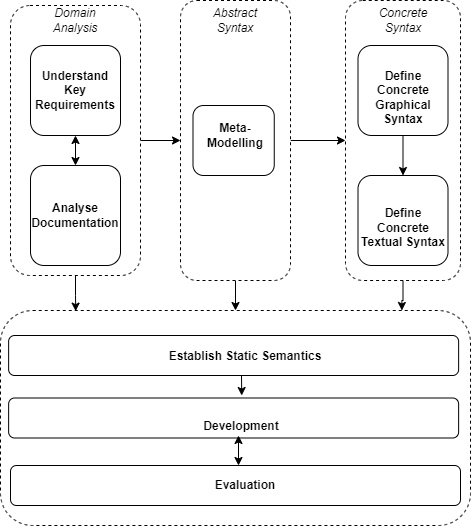
\includegraphics[keepaspectratio,height=9cm, width=12cm]{diagrams/methods.png}
\label{methover}
\end{figure}

\subsection{Performing Domain Analysis}
Prior to developing formalisms for our language, we identified key concepts that are relevant to the domain in which our language would be used i.e. variability management in the robotics. We also identified and clarified the purpose of our language as well as the stakeholders our activities are targetting. Finally, we identified all the relations between our gathered domain concepts which we derived from both stakeholders and relevant documentation, by studying the properties of our domain concepts.

\subsection{Implementation}
In our language implementation step, we define the capabilities of our language based on prior knowledge from our domain analysis and then conceived both the graphical and textual forms our language, to represent the syntactic structure of our language tokens. Graphically, we used feature models to define and model features of robot examples. On an abstract level, we used class diagrams to describe the capabilities present in our language.

\subsubsection{Defining the Abstract Syntax}
In creating the abstract syntax of our language, we formalised prior knowledge gathered in our domain analysis step into models. These models, otherwise known as meta-models were then refined in multiple iterations to reflect the requirements that form the capabilities of our variability-modelling language with respect to the problem space. We followed the following concrete steps to realise the abstract syntax of our language.\begin{enumerate*}
    \item Create a single decomposition of a class diagram together with compositional relationships.
    \item Verify the manner in which concepts are classified, and classes are organized in a hierarchy.
    \item Concretize relationships if need be. If relationships between concepts posses properties, they need to be transformed into classes.
    \item Remove redundancies by finding and removing multiple classes that have the same property.
    \item Evaluate resultant abstract syntax based on how accurately it reflects the problem and how well the concepts of design were kept within scope.
\end{enumerate*}

\subsubsection{Defining the Concrete Syntax}
The concrete syntax of our language is expressed both graphically and textually through feature models and JSON notation respectively. A major requirement of our implementation is to give potential users the expressive capability to create their own custom programs that will be in the form of modelled robotic features. In that, end users of our domain specific language have the ability to implement their own feature models of example robots that are adaptable in varying contexts. In a graphical context, feature models of example systems were conceptualised and implemented with FeatureIDE\foot{https://featureide.github.io/} and then further translated into JSON notation made up of multiple intuitive and configurable attributes.

\subsection{Establishing the Static Semantics}
After defining both the concrete and abstract syntax of our language, we proceeded to establish the static semantics of our language. The static semantics mentioned in this context, refers to the underlying rules that determine the validity of model variants that can be created with our language. Key aspects of the static semantics which we clarified and established include:
\begin{enumerate}
    \item Outlining mechanisms that realise static and dynamic binding.
    \item Describing the configuration space that defines the configurability of our model instances.
    \item Constraining the configuration space to limit the scope of adaptability.
\end{enumerate}

\subsection{Development}
In the development phase of our methodology, we utilised domain knowledge gathered from our domain analysis, concrete syntax definition, abstract syntax definition and static semantics as input to implement our domain specific language of the Python programming language. Our development approach can be summarized in the following steps:
\begin{enumerate}
    \item Gather system requirements by establishing the purpose of the language with regards to its functionality.
    \item Analyse requirements by transforming its specified textual functionalities into concrete functional and non-functional requirements.
    \item Establish design decisions such as the general architecture of the system, dependency management, choice of technologies and trade-offs, as well as implementation algorithms.
    \item Realise language designs with Python based algorithms and data structures. Likewise interfaces for integrating encapsulated feature implementations will be realised in  C++\foot{https://isocpp.org/}.
    \item Test implementation by evaluating the interactions of all the various integrated system components.
 \end{enumerate}
 
\subsection{Language Evaluation Overview}
Evaluating our language means to assess its implementation from three main perspectives. These perspectives include \begin{enumerate*}[label=(\roman*)]
\item Correctness,
\item Realizability and
\item Novelty.
\end{enumerate*}
\begin{itemize}
    \item \textbf{Correctness:} The validity of models and configurations created with our language along with the implied effect of a model's feature constraints are closely evaluated by both a schema and a constraint checker, which operate by detecting syntax and constraint violations.
    
    \item \textbf{Realizability:} Proof of realizability indicates that our binding technique which forms the core of our implemented variability mechanisms is feasible. This is quite relevant, given that modelling variability with feature binding time and binding mode has not yet been applied in robotics.
    
    \item \textbf{Novelty:} The novelty of our work is assessed along the lines of the innovative and conceptual uniqueness that defines the binding technique of our variability mechanism. By comparative positioning our study with other studies from the robotics domain, we would be in a position to back our claim of novelty through research.
\end{itemize}

By realising our variability modelling language to implement binding time and binding mode mechanisms in a manner that fulfils our research objectives, we were able to automatically provide proof of the realizability and novelty of our binding technique. In addition to this, a comprehensive evaluation plan was applied to test for type and syntax correctness.

\subsection{Correctness Evaluation}
As a functional requirement of our language, end users will have the means to build programs by modelling robotic features, defining configuration bindings for all modelled features, and applying configurations to multiple scenarios through implemented mechanisms. Configurations are typically an amalgamation of features, relationships and constraints. To be able to assess the validity of user defined configurations described with our language, we have implemented mechanisms that can be used to evaluate the well-formedness of both models and configurations. A high level description of our framework evaluation plan can be summarised as follows:
\begin{enumerate}
  \item Realise mock-ups of example robotic systems.
  \item Define configuration bindings for each mock-up example.
  \item Encapsulate and plug in source code implementations of defined mock-up features.
  \item Compile and validate the syntax and semantics of models and configurations.
  \item Execute and demonstrate model variability.
\end{enumerate}
For stakeholders to be able to verify the correctness of their models, all models and configurations defined with our modelling language must be validated on multiple levels of correctness i.e. syntax and semantic accuracy. 
\begin{itemize}[label={}]
  \item \textbf{Syntax Validation: }To effectively validate our language syntax, we evaluate the schemas of both model and configuration objects. Schema validation in this sense refers to token and token state validity.
 
  \item \textbf{Semantics Validation: } In out attempt to validate the semantic implications of our language, we assess the correctness of configuration bindings in relation to the corresponding binding constraints specified. We also judge the correctness of each configuration binding pair with respect to its implied effect on other features in a given configuration space.
  
\end{itemize}


\section{Results}
\subsection{Architectural Overview}
Our language, otherwise known as MoTiVML, is a lightweight variability modelling language which is structurally based on the Javascript Object Notation (JSON)\foot{https://www.json.org/json-en.html}, and implemented as a domain specific language of the Python programming language. Architecturally, this language consists of three modular components. These include a syntax manager, a configuration manager and a source code implementation manager. As shown in Figure \ref{arch-over}, all these components are encapsulated and offered as an open sourced ROS compatible framework.

The syntax manager component contains all implementations related to language tokens, as well as the language's lexical and syntactical schemas. Tokens in this sense, represent the legal keywords or lexemes that are permissible in our language. There are two decoupled schema representations offered in MoTiVML; a feature schema and a configuration schema. Language schemas are simply represented as an object of tokens mapped to selected data structures. Listing \ref{feat-schema} and \ref{bind-schema} show samples of a feature and configuration schema respectively.

\begin{listing}[H]
\caption{Feature Schema}
\begin{minted}[
framesep=2mm,
baselinestretch=1,
bgcolor=LightGray,
fontsize=\footnotesize,
showtabs=false,                  
tabsize=2
]{Json}

    {
        "id": "F0",
        "name": "ComponentControl",
            "constraints": {
	            "featuresIncluded": [],
	            "featuresExcluded": [],
	            "bindingTimeAllowed":"Early",
	            "bindingModeAllowed":"Static"},
        "group": "OR",
        "isMandatory": true
    }

\end{minted}
\label{feat-schema}
\end{listing}

\begin{listing}[H]
\caption{Configuration Schema}
\begin{minted}[
framesep=2mm,
baselinestretch=1,
bgcolor=LightGray,
fontsize=\footnotesize,
showtabs=false,                  
tabsize=2
]{Json}

{
    "id": "F0",
    "props": {
        "mode": "Static",
        "time": "Early"
    }
}
\end{minted}
\label{bind-schema}
\end{listing}

The configuration manager component of our library is made up of two parts. Namely, a binding semantics interpreter and a constraint checker. In general, variability management provides two main capabilities i.e. feature modelling and variation point definition and management. The binding semantics interpreter assimilates and displays the result of the interaction between the assigned binding pairs of any collection of features. The constraint checker on the other hand parses the entire model definition of an example system, to evaluate it for constraint violations in an attempt to validate user defined configurations with respect to the configuration space. Thus, the constraint checker enforces configuration rules that define the adaptability of configurations based on feature binding time and binding mode.
The source code implementation manager encapsulates a plug-in management interface which provides an integration point where end users can include source code implementations of modelled features into their configurations by wrapping them as self-contained plugins.

\begin{figure}[H]
\caption{Architectural Overview of Variability Management Solution}
\centering
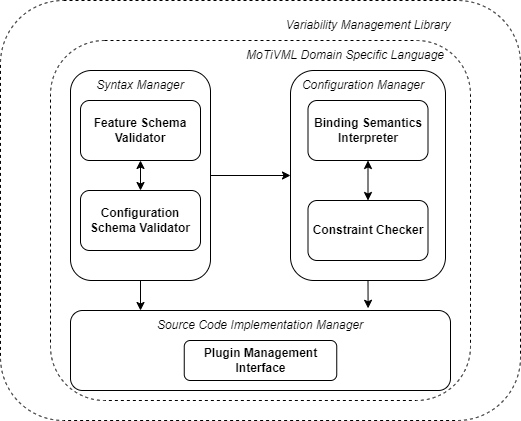
\includegraphics[width=0.5\textwidth]{diagrams/arch-overview.png}
\label{arch-over}
\end{figure}

\subsection{Domain Analysis}
In our language design, it was necessary for us to clarify key concepts that are relevant to the domain context of our language. Furthermore, we saw the need to identify design concepts and relationships that determine the type of programs which domain stakeholders will be capable of building with our language. All the concepts and relationships we identified, were then formalized into a model, and iteratively refined to develop our language's abstract syntax.

During our domain analysis phase, we identified five standard questions which make up the core ideas and knowledge base that represents our language and its use. These questions can be categorised as follows:
    \begin{itemize}
        \item \textbf{Purpose: } \textit{What is the purpose of this language?}\\
        The purpose of our language is to provide roboticists with means and techniques for planning, designing, and implementing variability through mechanisms, that implement binding time and binding mode techniques.
        \item \textbf{Stakeholders: } \textit{Who are the key stakeholders and the intended users of the language?}\\ Our language targets a very diverse group of skilled professionals in the robotics domain who can be classified as end users. These stakeholders/end users include 
        \begin{enumerate*}[label=(\roman*)]
            \item Operators: End users with minimal training on the usage of our framework, but have the ability to operate robotic applications with pre-configured configurations.
            \item Developers: End users in charge of developing, implementing and integrating new features into our framework.
            \item System Engineers: End users in charge of adapting the framework to match the specific requirements of a customer.
        \end{enumerate*}
        \item \textbf{Concepts: }\textit{What are the key domain concepts that targetted stakeholders care about?}\\ From an end user perspective, concepts such as simplified feature modelling techniques, standardized configuration management techniques and flexible yet customizable feature binding based on time and mode are key.
        \item \textbf{Relations: }\textit{How are domain concepts related, and what are their relevant properties?}\\
        Properties that define the core user concepts of our language include:
        \begin{itemize}
            \item Every instance of a feature class is selected by default.
            \item All features in a model are defined as mandatory by default upon instantiation.
            \item A parent feature may have zero or more child features.
            \item A modelled feature may have zero or more groups but a group must have two or more features to exist.
            \item A grouped set of features may belong to an OR or XOR group.
            \item A feature must have a binding time property which is set to \textit{Early} by default.
            \item A feature must have a binding mode property which is set to \textit{Static} by default.
            \item A modelled feature's binding time property can only exist in three states. i.e. \textit{Early, Late, Any}.
            \item A modelled feature's binding mode property can only exist in three states. i.e. \textit{Static, Dynamic, Any}.
        \end{itemize}
        \item \textbf{Examples: }\textit{What examples of language instances are available?}\\
        To the best of our knowledge, no language designed to model variability in robotic systems, using binding time and binding mode exists. Our language is built on novel principles crafted to effectively manage variability in ROS-based robotic systems.
    \end{itemize}
    
\subsection{Implementation}
In our architectural implementation, configuration capabilities are decoupled from feature capabilities. This is to primarily separate concerns by detaching feature attributes that do not require end user manipulation to form configurations from the ones that actually require it. Each set of decoupled configuration attributes references a corresponding feature by an \textit{ID} attribute.

\subsubsection{Developing Mock-up Examples}
An important use case of our language is that, it can be used to develop mock up examples that demonstrate the language's expressiveness. In the context of our study, examples refer to modelled features of robot product lines. Figure \ref{ex1} and \ref{ex2} show graphical representations in the form of feature models, of our selected example systems i.e. service robots. For each feature present in a model, we can express it textually with tokens from our language as shown in Listing \ref{feat-conc-text} and \ref{bind-conc-text}. Inspiration for these examples were drawn from general utility robots and disinfection robot product lines such as TIAGo and UVD Model C.
    
\begin{figure*}[h]
\caption{Modelled Example One}
\centering
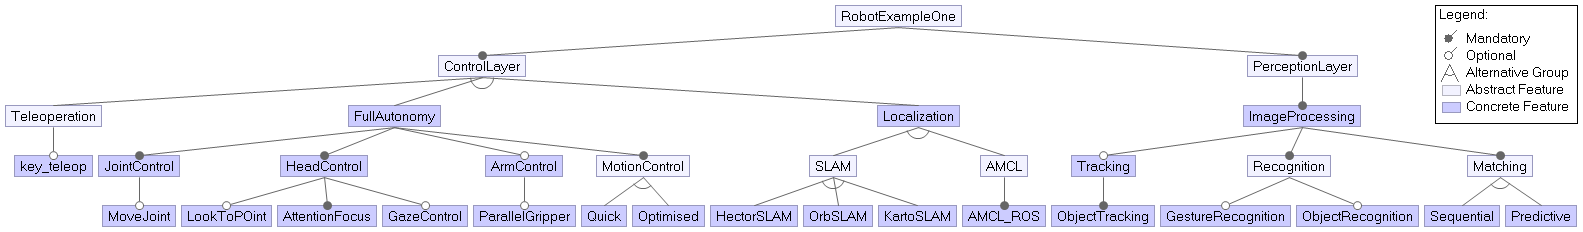
\includegraphics[width=0.9\textwidth,height=3cm]{diagrams/ex1.png}
\label{ex1}
\end{figure*}

\begin{figure*}[h]
\caption{Modelled Example Two}
\centering
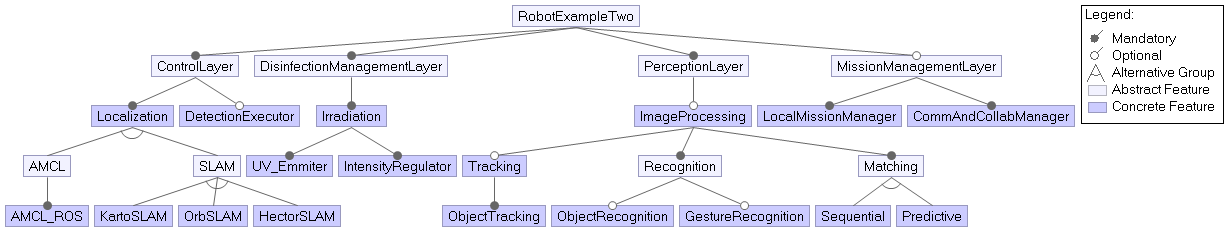
\includegraphics[width=0.9\textwidth,height=3cm]{diagrams/ex2.png}
\label{ex2}
\end{figure*}
    
Furthermore, in our model refinement step, that aims at extending our mock-up examples against our requirements, we analyse the requirements associated with our language, justify if these requirements are met and then proceed to provide examples or evidence of said requirements that have been fulfilled.

\begin{listing}[H]
\caption{Textual Sample of Features}
\begin{minted}[
framesep=2mm,
baselinestretch=1,
bgcolor=LightGray,
fontsize=\footnotesize,
showtabs=false,                  
tabsize=2
]{Json}
{
    "id": "root_feature",
    "name": "simpleBot",
    "group": "",
    "isMandatory": true,
    "sub": [
	        {"id": "F0",
	        "name": "ComponentControl",
	        "constraints": {
		        "featuresIncluded": [],
		        "featuresExcluded": [],
		        "bindingTimeAllowed":"Early",
		        "bindingModeAllowed":"Static"},
	        "group": "OR",
	        "isMandatory": true
	        "sub":[
	            {
	            "id": "F1",
	            "name": "..."
	            }
	        ]
        }
    ]
}
\end{minted}
\label{feat-conc-text}
\end{listing}

All features present in our feature model specification posses binding time and binding mode configurations which can be used by our language to manage variability within a modelled robotic system. As indicated in our architectural design, configuration collections are separated from feature collections for the sole purpose of decluttering model documents by abstracting configuration attributes from the main set of feature attributes. Listing
\ref{bind-conc-text} captures a sample representation of the concrete textual syntax of feature configurations present in a given model. This consists of a collection of feature \textit{ids} together with their \textit{time} and \textit{mode} binding properties, derived from a separate collection of feature documents nested in the same order as their corresponding graphical feature model.

\begin{listing}[H]
\caption{Textual Sample of Feature Configurations}
\begin{minted}[
framesep=2mm,
baselinestretch=1,
bgcolor=LightGray,
fontsize=\footnotesize,
showtabs=false,                  
tabsize=2
]{Json}
{
	"properties": [
	    {
	    "id": "F0",
	    "props": {
	        "mode": "Static",
	        "time": "Early"
	    	}
	    },
	    {
	    "id": "F1",
	    "props": {
	        "mode": "Static",
	        "time": "Early"
	    	}
	    }
	]
}
\end{minted}
\label{bind-conc-text}
\end{listing}

\subsubsection{Extending Mock-up Examples Against Requirements}
In our domain analysis we were able to understand key requirements relevant to our language's desired capabilities. Based on this understanding, we extended our mock up examples in Figure \ref{ex1} and \ref{ex2} against our already established language requirements. Such established language requirements include:
\begin{enumerate}
    \item R1: End users can instantiate robotic models.
    \item R2: End users can create instances of features within models.
    \item R3: End users can create decoupled model configurations.
    \item R4: End users can define and link configurations to feature instances.
    \item R5: End users can evaluate models both syntactically and semantically.
\end{enumerate}
Using the concrete textual syntax of our modelling language which we have highlighted in Listing \ref{feat-conc-text} and \ref{bind-conc-text}, we identified example syntax representations that fulfil all the requirements listed above. Table \ref{tab:reqext} captures a mapping of each requirement along with its example syntax representation, that justifies that a requirement has been fulfilled.

\begin{table}[H]
\caption{Extended Mock-up Examples Against Requirements}
\begin{center}
\begin{tabular}{|c|c|}
\hline
    Requirement & Example Syntax  \\ \hline
     R1 & \multirow{2}{*}{$\{"id":"root\_feature","name":"simpleBot",$}\\
                        & \\
                        & $"group": "","isMandatory": true,"sub": []\}$\\ \hline
     R2 & \multirow{2}{*}{$\{"id": "F1","name": "Localization",$}\\ 
                        & \\
                        & $"constraints": \{"featuresIncluded": [],$\\ 
                        & $"featuresExcluded": [],$\\
                        &$"bindingTimeAllowed":"Early",$ \\
                        & $"bindingModeAllowed":"Static"\},$\\ 
                        & $"group": "","isMandatory": true\}$ \\
                         \hline
     R3 &  \multirow{2}{*}{$\{"id": "F1","props": \{$}\\
            & \\
            & $"mode": "Static","time": "Early"\}\}$\\
            & \\
            \hline
     R4 & $"props": \{"mode": "Static","time": "Early"\}\}$\\ \hline
     R5 & \multirow{2}{*}{Using the schema and constraint checker,}\\ 
        & \\
        & syntax, grammar and semantics of a model can be evaluated\\ \hline
\end{tabular}
\label{tab:reqext}
\end{center}
\end{table}

\subsubsection{Identifying Language Tokens}
The basic compositional unit of our language is an attribute. From a lexical standpoint, these attributes are derived from a defined set of legal or permissible keywords referred to as tokens. These tokens form part of a key-value pair production. Tokens can be identified and extracted from the key-value pair attributes that make up a feature in our model and configuration collections. Attribute keys serve as meta-data for the data held by their corresponding values. Table \ref{tab:langlex} shows all identified tokens together with the regular expressions that define their legal or valid lexical structures.

In Table \ref{tab:langlex}, for each identified token in our language, we translated a valid representation of it into a regular expression to demonstrate which valid forms of these token can exist in our language. Syntactically speaking, modelled features and their configurations, encapsulate key-value paired attributes as self-contained objects. Lastly, Table \ref{tab:langlex} also captures a list of generated terminal symbols that can be used in grammar production.

\begin{table}[H]
\caption{Language Tokens}
\begin{center}
\begin{tabular}{|c|c|c|}
\hline
    Token & Regular Expression & Terminal Symbol \\\hline
                             id & 'id' & Id  \\\hline
                             name & 'name' & Name \\ \hline
                             featuresIncluded & 'featuresIncluded' & FeaturesIncluded\\ \hline
                             featuresExcluded & 'featuresExcluded' & FeaturesExcluded\\ \hline
                             bindingTimeAllowed & 'bindingTimeAllowed' & BindingTimeAllowed\\ \hline
                             bindingModeAllowed & 'bindingModeAllowed' & BindingModeAllowed\\\hline
                             group & 'group' & Group\\ \hline
                             isMandatory & 'isMandatory' & IsMandatory\\ \hline
                             time & 'time' & Time\\ \hline
                             mode & 'mode' & Mode\\ \hline
                              "Early" & 'Early' & Early\\ \hline
                              "Late" & 'Late' & Late\\ \hline
                              "Static" & 'Static' & Static\\ \hline
                              "Dynamic" & 'Dynamic' & Dynamic\\ \hline
                              "Any" & 'Any' & Any\\ \hline
                              "true" & 'true' & True\\ \hline
                              "false" & 'false' & False\\ \hline
                              "OR" & 'OR' & OR\\ \hline
                              "XOR" & 'XOR' & XOR\\ \hline
                              alphaValue & $(a-zA-Z)^+$ & alphaVal\\ \hline
                              %alphanumValue & $(a-zA-Z0-9)^+$ & anumVal\\ \hline
                              boolValue & $[true | false]$ & boolVal\\ \hline
\end{tabular}
\label{tab:langlex}
\end{center}
\end{table}

\subsubsection{Specifying Language Terminals}
Our language's syntax can be described as a production consisting of left-hand-side and right-hand-side attributes. For each attribute, the left-hand-side consists of non-terminals that serve as language meta-data. On the right-hand-side however, we can identify singular or grouped forms of terminal and non-terminal symbols in the form of data. Left-hand-sided and the right-hand-sided attributes are separated by a colon (:) and each model attribute in turn is separated from the next by a comma(,). Table \ref{tab:langlex} captures all meta-data and data tokens that define our language.

\subsubsection{Identifying Syntactic Categories Within Our Language}
The modelling capability of our language provides domain stakeholders with a means of instantiating a feature model, as well as the possibility of defining and configuring features. Within our language's concrete syntax, one implicit and two explicit syntactic categories can be identified. These categorizations include:
\begin{enumerate}
    \item \textit{Feature Description Block:} This is made up of all feature attributes that are concerned with describing the general purpose of a feature. Although this category is not explicitly expressed in the textual formalism of a feature's schema, it can still be defined as a set of individual feature attributes which intuitively provide descriptive contexts to the functionality and purpose of a feature.
    \item \textit{Constraints Block:} This is represented as a nested block of feature attributes that define the type constraints applicable to a feature as well as the set of possible constraint values that are valid for that feature.
    \item \textit{Binding Properties (props) Block:} For every feature, there exists a corresponding configuration. Within the configuration of a feature exists a binding property block definition. The purpose of this binding property block is to allow domain stakeholders to configure binding time and binding mode attributes for each feature they define. These binding time and binding mode attribute definitions serve as the fundamental variation mechanism for each feature model.
\end{enumerate}
 
\subsubsection{Specifying Grammar Rules} By combining the terminals defined in Table \ref{tab:langlex} with the syntactic categories identified in the previous section, we were able derive grammar productions for our language. The grammar rules present in our language for all three syntactic categories can be expressed as follows:\\

\begin{itemize}
	\item[] featureDescriptionBlock $\longrightarrow$ '\{'\ 'id'\ ':'\ alphaVal,\ 'name'\ ':'\ alphaVal,\ 'group'\ ':'\ alphaVal, 'isMandatory'\ ':'\ boolVal\ '\}' \\
	
	\item[] constraintsDefinitionBlock $\longrightarrow$ constraints: '\{'\ 'featuresIncluded'\ ':'\ '['\ Id, Id, ...\ ']',\ 'featuresExcluded'\ ':'\ '['\ Id, Id, ...\ ']',\ 'bindingTimeAllowed'\ ':'\ alphaVal,\ 'bindingModeAllowed'\ ':'\ alphaVal '\}'\\
	
	\item[] bindingPropertiesBlock $\longrightarrow$ '\{'\ 'time'\ ':'\ alphaVal,\ 'mode'\ ':'\ alphaVal '\}'\\
\end{itemize}

\subsubsection{Abstract Syntax Definition}
The abstract syntax of any language refers to the logical representation of that language in memory. In Figure \ref{femet} and \ref{conmet} we provide an abstraction to the user interfaces of both a feature and a configuration objects in the form of class diagrams. Upon instantiation, a feature is selected by default. By design, every modelled feature must bear a unique \textit{id} string attribute which serves as a reference point throughout multiple points in our implementation. Every feature bears a \textit{name} that describes its intended purpose and capability.

Furthermore, every feature has a set of constraints which define the scope of the feature in the model configuration space. Feature constraints are categorised into two main groups. i.e. cross functional constraints and binding property constraints.  Cross functional constraints refer to \textit{includes} and \textit{excludes} constraints while binding property constraints define the possible state values of binding time and binding mode attributes within configurations. A feature may contain an aggregation of sub-features. On the other hand, every feature is composed if a group, which may comprise of strictly two or more features.

\begin{figure}[H]
\caption{Feature Meta Model}
\centering
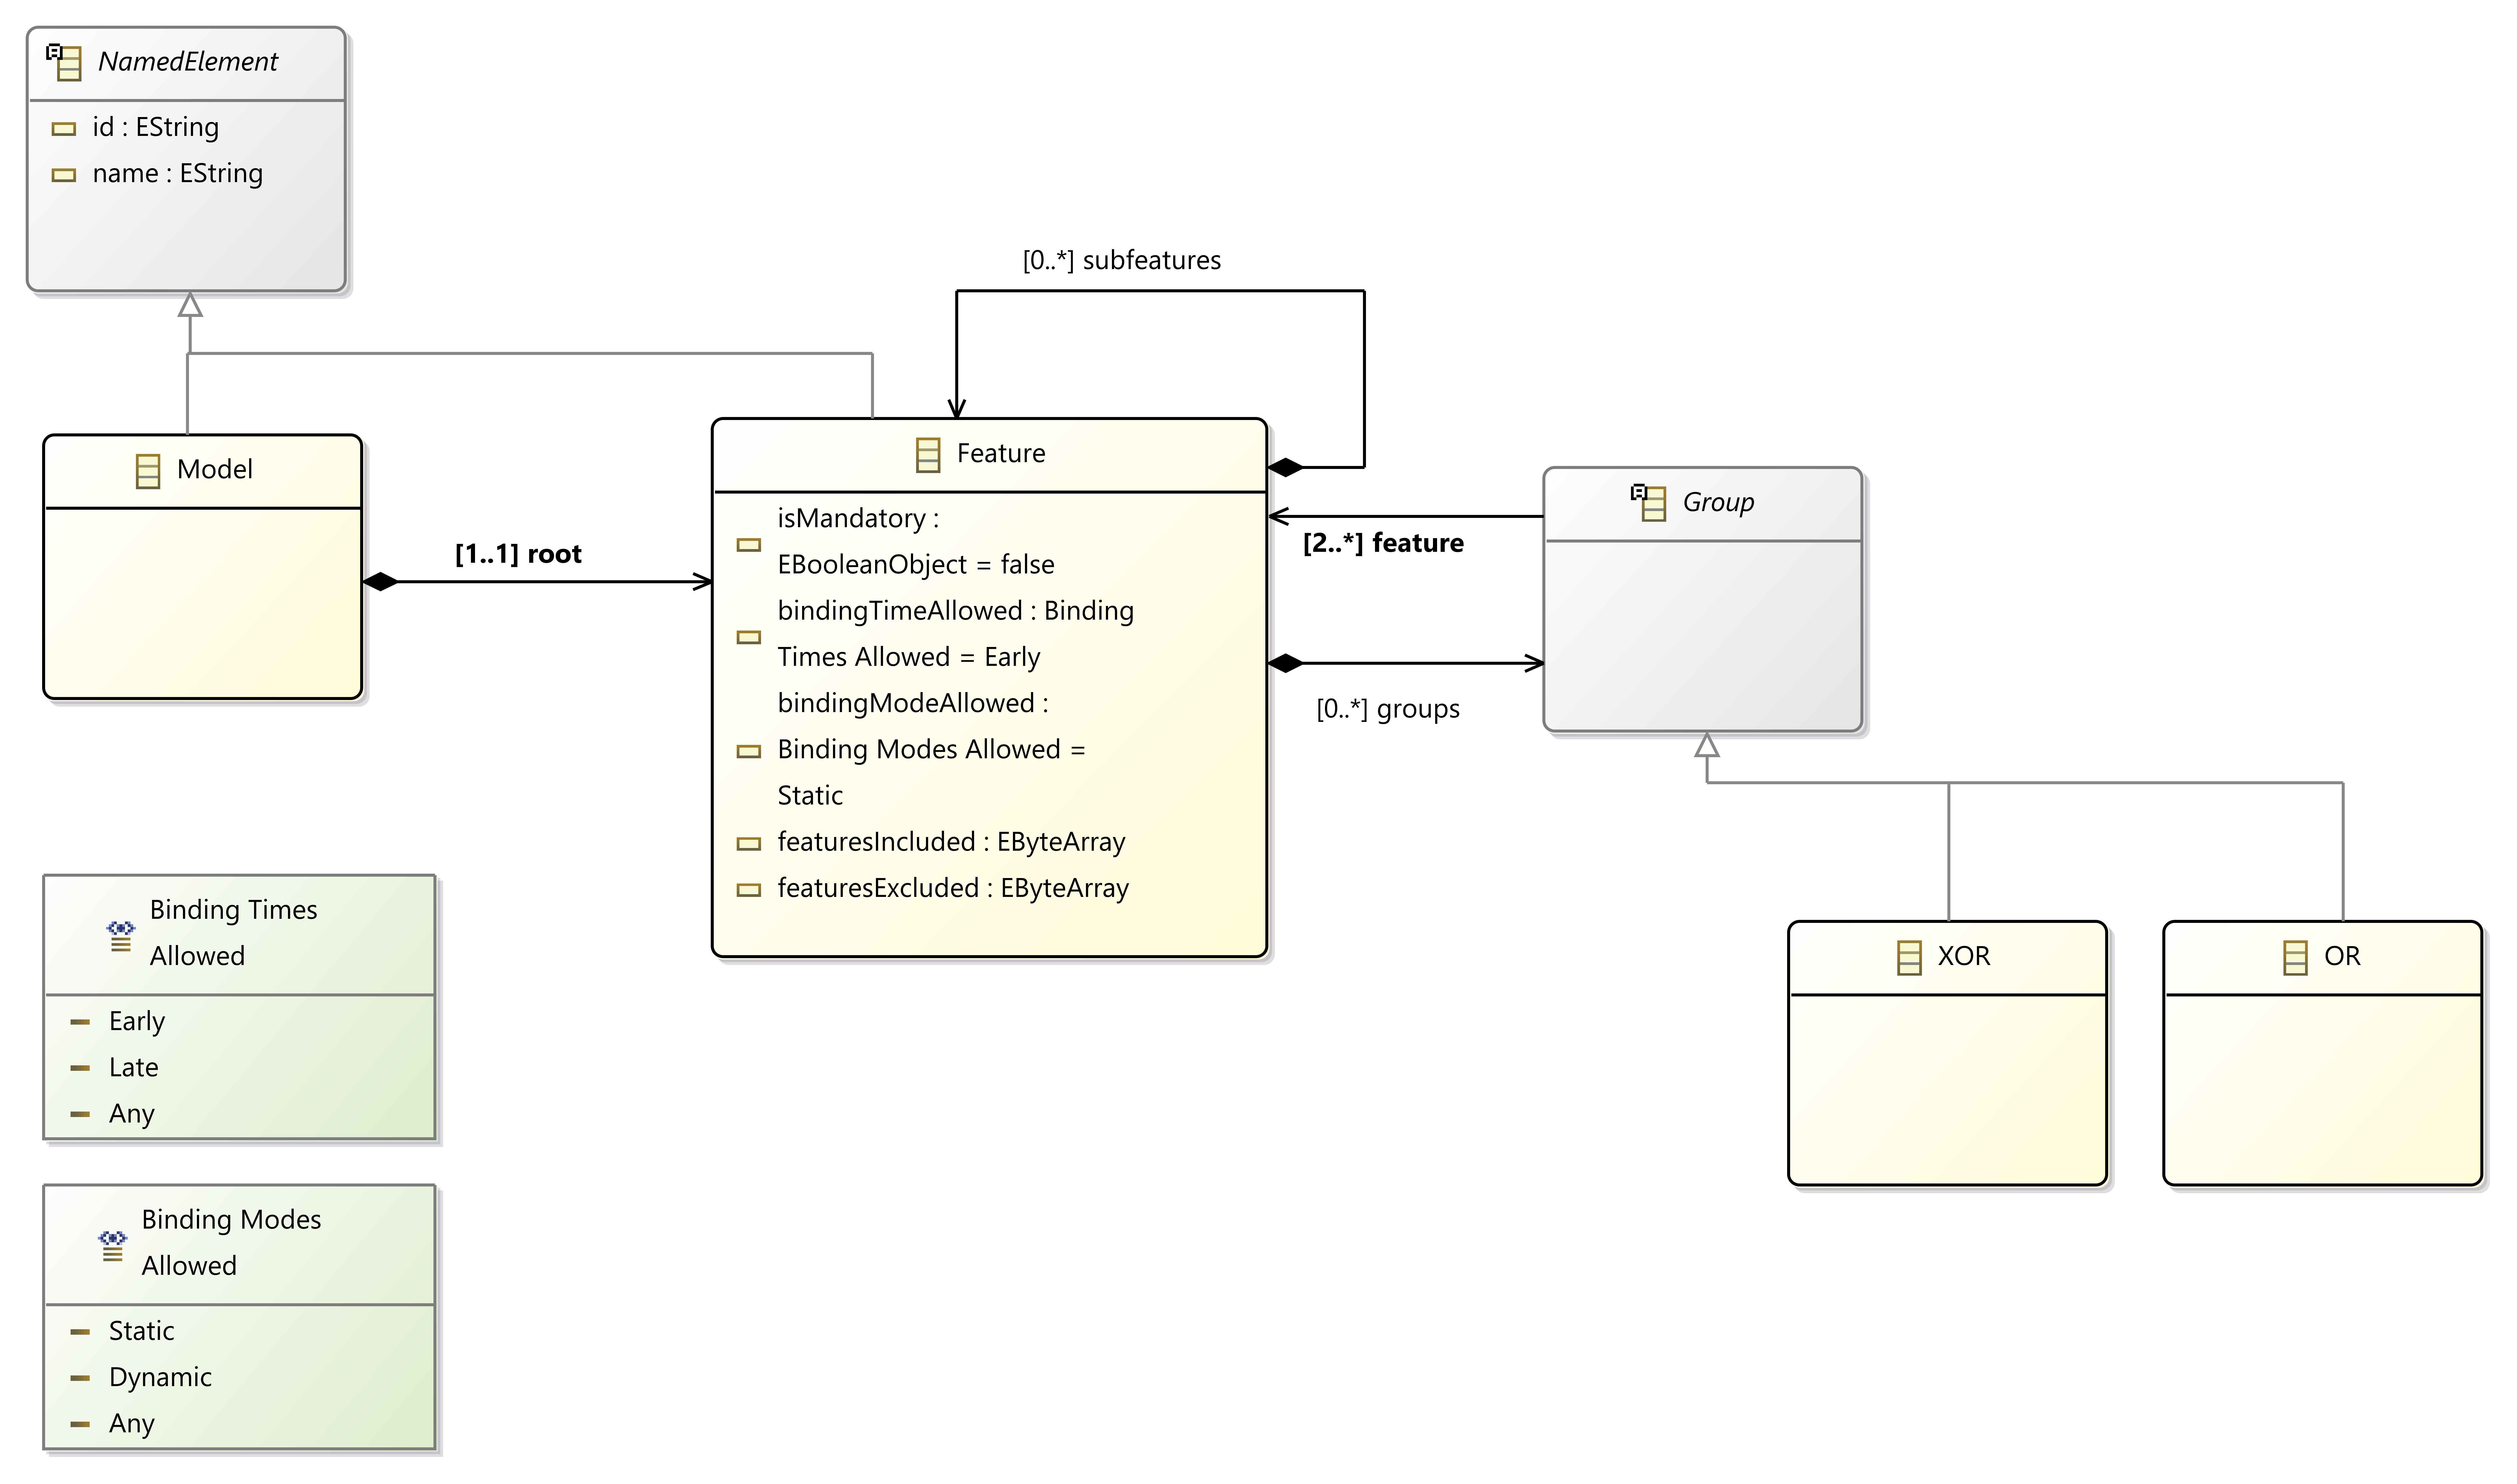
\includegraphics[width=0.5\textwidth]{diagrams/feature.png}
\label{femet}
\end{figure}

The configuration capabilities of a feature reflects the ability of the feature to be adapted to fit multiple contexts. Per our proposed variability management technique,
feature adaptations are determined by a binding time and binding mode combination, specified or assigned based on end user preferences. Each configuration bears reference to an existing feature by way of an \textit{id} attribute. For each feature, its multiplicity can be described as one or more. Thus, there can exist multiple configurations, provided these configurations are valid with respect to the feature constraints. In each encapsulated instance of a model, it can be observed in Figure \ref{conmet} that configurations are represented as feature compositions. Also, model, feature and configuration functionalities can be generalised into a single named element. 

\begin{figure}[H]
\caption{Configuration Meta Model}
\centering
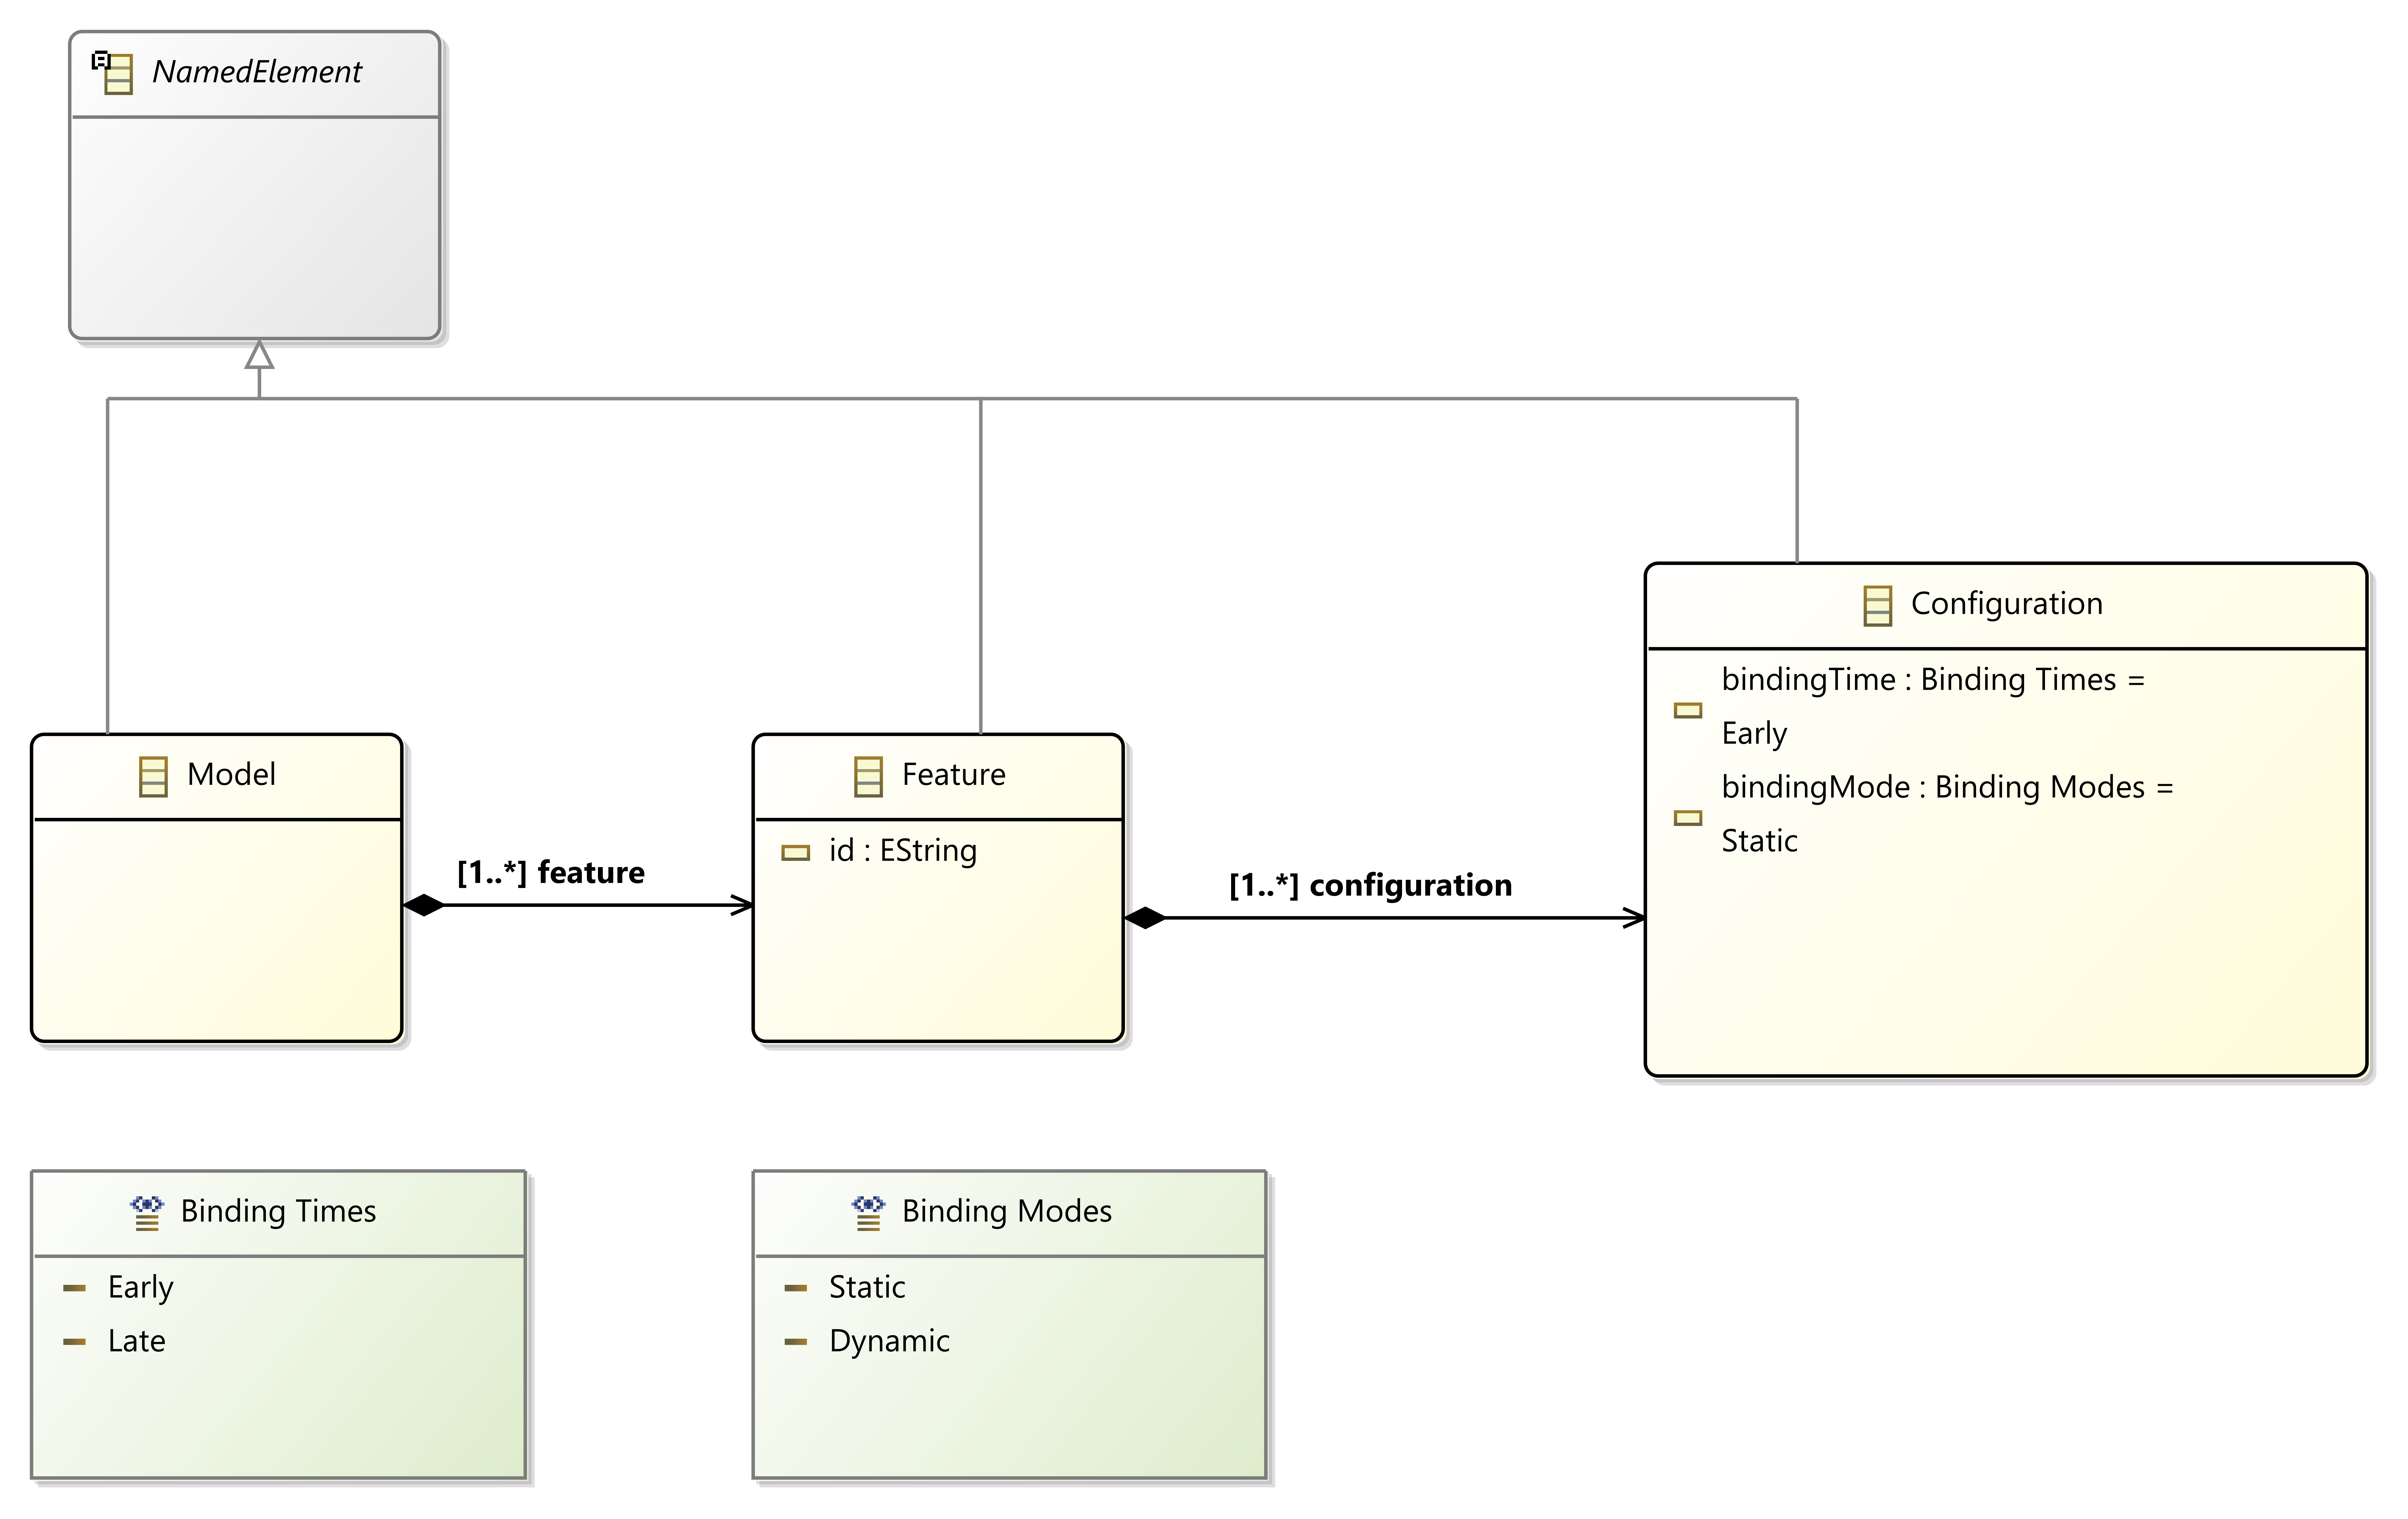
\includegraphics[width=0.5\textwidth]{diagrams/config.png}
\label{conmet}
\end{figure}

\subsubsection{Identifying Binding Mechanisms}
Realising static, dynamic, early and late bindings in robotic applications can be tricky due to minor inconveniences related to compatibility. For both time and mode based binding, there are  ROS based implementations in both C++ and Python, that can be used to realise this.

In Table \ref{tab:realmecha}, we have highlighted some of such implementations, otherwise known as mechanisms, which we used to realise all possible binding pairs found within our configuration space. These include, the C++ preprocessor for static, ROS pluginlib for dynamic and ROS parameters together with roslaunch for early and late binding.

\begin{table}[H]
	\caption{Static and Dynamic Binding Mechanisms}
	\begin{center}
		\begin{tabular}{|c|c|}
			\hline
			Binding Type & Binding Mechanism \\ \hline
			Static & C++ preprocessor \\ \hline
			Dynamic &  ROS Pluginlib  \\ \hline
			Early \& Late &  roslaunch , ROS parameters  \\ \hline
			
		\end{tabular}
		\label{tab:realmecha}
	\end{center}
\end{table}

\subsubsection{Implementing Binding Mechanisms}
The binding mechanisms mentioned in Table \ref{tab:realmecha} serve as unique implementation techniques that provide our modelling framework with the capability to handle variability on an implementation level. In that, modelled variation points of robot instances that have been described and implemented with our framework, are able to leverage such techniques through ROS, to demonstrate static, dynamic, early and late binding of implemented features within all user defined programs.

Furthermore, these integrated mechanisms are robust open source implementations that are compatible across a number of platforms. Thus, by utilising their capabilities, we were able to create both flexible and customizable configuration properties through our feature bindings.
\begin{itemize}
	\item \textbf{C++ Preprocessor for Static Binding:}
	\begin{listing}[H]
		\caption{Examples of Static Feature Inclusions}
		\begin{minted}[
			framesep=2mm,
			baselinestretch=1,
			bgcolor=LightGray,
			fontsize=\footnotesize,
			showtabs=false,                  
			tabsize=1
			]{cpp}
			#ifdef AMCL
			#include "../../featx/Amcl.h"
			#endif
			
			#ifdef MTNPLNCTRL
			#include "../../featx/MotionPlanningCtrl.h"
			#endif
			
			#ifdef COMPCTRL
			#include "../../featx/ComponentControl.h"
			#endif
		\end{minted}
		\label{cpp-static}
	\end{listing}

Within our implementation, we have a designated static feature loader module that executes a series of conditional statements in the form of preprocessor directives to determine which features are to be included or excluded at compile time. As shown in Listing \ref{cpp-static} above, implemented feature classes \textit{Amcl.h}, \textit{MotionPlanningCtrl.h} and \textit{ComponentControl.h} will be included in our user program build if they are explicitly defined as part of the configuration. This mechanism exists strictly for static features that are loaded at compile time.

For static feature loaded at runtime, we implemented a customised plugin-type mechanism which disallows changing a said feature after it has been loaded at runtime.

\item \textbf{ROS Pluginlib for Dynamic Binding:}
	\begin{listing}[H]
		\caption{Examples of Dynamic Feature Plugin Implementations}
		\begin{minted}[
			framesep=2mm,
			baselinestretch=1,
			bgcolor=LightGray,
			fontsize=\footnotesize,
			showtabs=false,                  
			tabsize=2,
			breaklines
			]{cpp}
		PLUGINLIB_EXPORT_CLASS(motivml_plugins::Slam, plugin_base::PluginInterface)
		
		PLUGINLIB_EXPORT_CLASS(motivml_plugins::Hands, plugin_base::PluginInterface)
		
		PLUGINLIB_EXPORT_CLASS(
		motivml_plugins::Pointscloud, plugin_base::PluginInterface)
		
		PLUGINLIB_EXPORT_CLASS(
		static_integration::Amclros, static_base::StaticInterface)
		\end{minted}
		\label{pluginlib-dynamic}
	\end{listing}

To simulate dynamic binding in general, we used the ROS pluginlib mechanism to encapsulate feature classes as plugins. Our choice use ROS pluginlib was influenced by the fact that it is lightweight, robust, stable and easy to integrate as a third party library. In addition, it comes with a very intuitive documentation\foot{http://wiki.ros.org/pluginlib} backed by an active community of contributors.

Listing \ref{pluginlib-dynamic} demonstrates how the ROS version of the pluginlib library is used to export classes that can later be consumed by programs as plugins.

\item \textbf{ROS Params and roslaunch for Time Binding:} On the ROS parameter server of our application, a categorised set of lists containing all bindings of a given robot instance, is stored to be able to categorically load these features at specific points i time upon the execution of the \textit{roslaunch} command.
\end{itemize}
\subsubsection{Integrating Binding Mechanisms Into Framework Components}
To provide roboticists with a SERA integrated solution that has the means
and techniques to implement variability, we integrated our implemented binding mechanisms on a component level into out framework solution.  Figure \ref{mecha-compo} shows the component interaction between our variability modelling language and our robot builder component on ROS. To complement this, we have provided a brief description of our chosen mechanisms with respect to their functions below.

\begin{figure}[H]
	\caption{Binding Mechanisms Component Diagram}
	\centering
	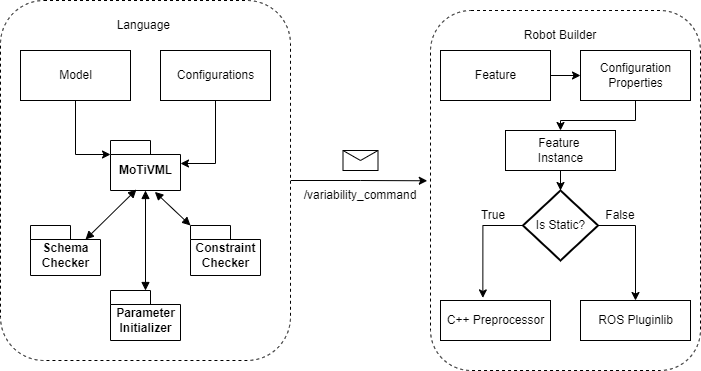
\includegraphics[width=0.5\textwidth]{diagrams/mecha-compo.png}
	\label{mecha-compo}
\end{figure}

\begin{itemize}
	\item \textit{Language Component: }
	The language component of our variability management framework, enables domain stakeholder to translate feature models into MoTiVML object models where time and mode bindings can be defined with constraints. In addition to that, our language provides both a schema and constraint checker purposefully for validating user defined models for syntactic and semantic correctness respectively. Furthermore, the language component contains a parameter initializer which instantiates and initializes ROS parameters used by our framework to enforce time based binding.
	\item \textit{Robot Builder Component: }
	The robot builder component of our framework is a ROS node within our source code implementation manager, that provides interfaces through which class implementations of registered features in our user defined models can be bound. It listens for configuration commands from the MoTiVML language interface over a ROS topic. For statically bound features, the C++ preprocessor together with conditional statements are used to include or exclude feature classes to and from robot programs.  In the case of dynamic binding, the ROS pluginlib library is used to register, encapsulate, export and load feature classes dynamically into prebuilt robot programs. Finally, this component also reads from initialised ROS parameters to retrieve and classify program features into time based categories. 
\end{itemize}


\subsection{Static Semantics}
In the compile time state of our variability modelling language, program syntax is evaluated based on internally established feature relationships and constraints that define the static semantics of our language.

The scope of our static semantics, which can be verified  at compile time, includes data type evaluation i.e. whether or not all tokens have been declared, which token declaration applies to which instances and so on. When it comes to controlling the semantic scope, constraint type declaration and implementation as well as the model level effect of constraints on each other can be inferred from feature interaction in a configuration.

\subsubsection{Describing the Configuration Space}
As shown in the concrete syntax of our feature modelling language, every instance of a feature has a binding time and binding mode attribute assigned to it. The interaction that occurs between these binding attributes, exits in a scope known as the configuration space. Within this scope, each feature possess dependencies and constraints that validate or invalidate defined feature instances. With the aid of propositional logic, table \ref{tab:propmap} provides a description of all likely dependencies and constraints of any given model instance. Per the results displayed in table \ref{tab:propmap}, mandatory features exhibit a bidirectional logical relationship between features indicating that both features require or depend on each other in all instances in which they are implemented. Conversely, an optional feature indicates a unidirectional behaviour between a parent and child feature, where a child feature may imply a parent feature but the parent feature on the other hand can exist without that child feature. For cross-functional constraints in the form of inclusions and exclusions, feature inclusion translate to an implication constraint while exclusion could be represented as  A $\Rightarrow$ $\neg$ B \ or \ $\neg$ (A $\land$ B).

\begin{table}[H]
\caption{Propositional Logic Mapping for Feature Model Attributes}
\begin{center}
%\begin{tabular}{|c|c|c|}
\begin{tabular}{|P{2cm}|P{2cm}|P{2cm}|}
\hline
    Attribute Name & Feature Model Notation & Propositional Logic  \\ \hline
    Mandatory & 
\vspace{0.3px}    
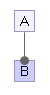
\includegraphics[width=10mm, height=12mm]{diagrams/mandatory.png} & A $ \Leftrightarrow $ B \\ \hline
    Optional &\vspace{0.3px} 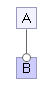
\includegraphics[width=10mm, height=12mm]{diagrams/optional.png}  & A $ \Rightarrow $ B \\ \hline
    Includes (requires) & A implies B &  A $ \Rightarrow $ B \\ \hline
    Excludes & A implies (Not B) &  A $ \Rightarrow $ $ \neg $ B \\ \hline
\end{tabular}
\label{tab:propmap}
\end{center}
\end{table}

The underlying logic of this language design requires the interaction of a feature's binding attributes, that serves as a variation mechanism for all feature models defined with this language. Table \ref{tab:timoconf} captures the semantics of possible binding time and binding mode combinations in any given model. This is relevant because, analysing the combined semantic effect of possible binding pairs in a model, gives insight into the feasibility or validity of combinations in the configuration space. Using propositional logic, Table \ref{tab:timoconf} shows the results of every possible interaction between binding pairs with respect to feature attributes such as mandatory, optional, includes and excludes. 

\begin{table}[H]
\caption{Feature Model Binding Semantics: \textbf{S = Static, E = Early, L = Late, D = Dynamic}}
\begin{center}
\begin{tabular}{|c|c|c|c|c|c|}
\hline
    A & B & B $ \Rightarrow $ A & A $ \Rightarrow $ B & A $ \Leftrightarrow $ B \\\hline
         SE & SE & 1 & 1 & 1  \\ \hline
         SE & SL & 1 & 0 & 0  \\ \hline
         SE & DE & 1 & 0 & 0 \\ \hline
         SE & DL & 1 & 0 & 0 \\ \hline
          
         SL & SL & 1 & 1 & 1 \\ \hline
         SL & DE & 0 & 0 & 0 \\ \hline
         SL & DL & 1 & 0 & 0 \\ \hline
         
         DE & DE & 0 & 0 & 0 \\ \hline
         DE & DL & 0 & 0 & 0 \\ \hline
         
         DL & DL & 0 & 0 & 0 \\ \hline
         
\end{tabular}
\label{tab:timoconf}
\end{center}
\end{table}

\subsubsection{Constraining the Configuration Space}
As part of our static semantics definition to confine our configuration space, we enforced a number of feature level constraints. To implement this, we conceived a number of ground rules or pre-conditions and enforced them as part of our modelled feature capabilities, to serve as our means of managing the scope of robot product lines that can be modelled with our solution. Additionally, we provide a means of validating a feature's constraint settings via an in-built constraint checker mechanism, that parses and interprets configuration attributes, to identify possible constraint violations. The different types of constraints that exist in our language, their purpose, together with their cumulative effect on each other, are described as follows.
\begin{itemize}
    \item \textit{Inclusion Constraint: }
    Otherwise referred to as an implies constraint, satisfies the condition that a given robotic feature tends to require others to function. For example, supposing there are two features \textbf{A} and \textbf{B}, \textbf{A} \textit{includes} \textbf{B} would imply that, if feature \textbf{A} is selected, feature \textbf{B} must also be to be selected.
    %% give examples
    
    \item \textit{Exclusion Constraint: }
    Some robotic features on the other hand do not require others to function We express this as an excludes constraint in our implementation. Again, supposing there are two features \textbf{A} and \textbf{B}, \textbf{A} \textit{excludes} \textbf{B} would imply that when feature \textbf{A} is selected, feature \textbf{B} cannot be selected and vice versa.
    
    
    \item \textit{Sub Feature Constraint: }
    Given the fact that the capabilities specified in our abstract syntax definition supports a hierarchical parent-child relationship amongst modelled features, a feature with a \textit{static} mode cannot exist as a child of a \textit{dynamic} parent. Allowing that form of inheritance would imply that an unloaded parent feature would create an orphan child feature, leading to the phenomenon of unused features stuck in runtime. 
    

\item \textit{Binding Property Constraints: }
As shown in our feature meta-model, the binding time and binding mode attributes of a feature are constrained to a set of valid inputs. By defining a set of valid binding time and mode input values, we are able to constrain the main feature attributes of user defined feature model instances.

\begin{table}[htbp]
\caption{Valid Binding Property Values}
\begin{center}
\begin{tabular}{|c|c|}
\hline
    Binding Property & Allowed State Values  \\ \hline
    Binding Time & Early, Late, Any \\ \hline
    Binding Mode & Static, Dynamic, Any\\ \hline
\end{tabular}
\label{tab:bpropcon}
\end{center}
\end{table}

\begin{itemize}
    \item \textit{Binding Time:} The binding time attribute of a feature can assume three distinct values. Binding times can be set to \textit{early}, \textit{late} or \textit{any}. This means that features can either be strictly bound at compile time, strictly bound at runtime or can alternate between compile time and runtime state values.
    
    \item \textit{Binding Mode:} The binding mode attribute of a feature can assume three distinct values as well. It can either have a \textit{static}, \textit{dynamic} or an \textit{any} value. This implies that a feature can either be strictly static, strictly dynamic or in the case of an \textit{any}, a feature can alternate between static and dynamic mode states.
\end{itemize}

\end{itemize}

\subsection{Implementing Defined Features}
As an extension to our modelling language, users do not only have the capability of defining and modelling features, but can also integrate source code implementations of features into their models. Through our provided language-agnostic interface, extracted source code implementations of features can be encapsulated and integrated into our library, where they can be referenced based on mechanisms provided within our implementation.

\section{Validation}
For us to be able to thoroughly validate our language design and its implementation, we have to ensure that we are able to evaluate user generated artifacts realised with our variability modelling language. These artifacts can be identified as feature models and configurations which contain both data and meta-data. To demonstrate this, we translated graphical representations of our mock-up examples in Figure \ref{ex1} and \ref{ex2} into model and configuration instances of our language. We then went on to validate the models and configurations for syntax and semantic correctness or well-formedness. Validation mechanisms used for syntax and semantic validation include a schema and constraint validation tools. The schema validation tool is used to evaluate model schemas of all features and configurations, whereas the constraint validator handles the semantic evaluation of bindings defined within our mock-up examples.

  \subsection{Schema Validation Tool} Our library provides a schema validation tool which certifies that the grammar and syntax rules of programs created with our language are structurally valid. Using our language, features and configurations can be conveniently modelled as key-value pairs of objects. Grammatically, a feature's object keys are represented as tokens that are not only terminal in nature, but also store meta-data on the features they represent. Value tokens on the other hand are generated from a finite set of data types which are unique to each object attribute present within a feature.
  
  The operations of our in-built schema validation tool can be classified into two categories. i.e. feature schema validation and configuration schema validation. Feature schema validation demands that a feature's model meta-data is validated by checking for absent or misrepresented tokens. A configuration on the other hand is validated based on meta-data such as its \textit{id}, \textit{binding time} and \textit{binding mode} properties. In both cases however, in the event of an absent or misrepresented token, an invalid schema error is triggered in the form of a console prompt, indicating the specific feature that bears the error.
  
  \subsection{Constraint Validation Tool} Embedded within our library is another component referred to as the constraint validator. This implementation, purposefully evaluates the semantic implications of each feature's constraints against its configuration settings, in the grand scheme of the configuration space. Our constraint validator tool, operates by parsing and interpreting feature models to validate two main types of semantics. The first is the set of configurations that have been defined within the scope of the constraints enforced. The second is the validity of configuration binding pairs with respect to other binding pairs within a specified product line definition.
  
 This capability of our library, backs the claim that our binding technique is flexible and customizable. An as such can be used to adapt product lines to fit varying usage contexts.

By evaluating our language with respect to the challenges and the research questions we have previously highlighted in Section \ref{section:intro}, we can therefore assess the degree to which domain challenges that have driven this study have been fulfilled. In subsequent sections, we analyse each domain challenge in close alignment with our research goals to further prove the relevance of our research outcomes.

\subsection{Lack of a Standard Variability Modelling Framework}
This challenge is addressed by the core mechanism that defines variation point implementations of models in our framework. In our light-weight architecture, features in a model can be modelled, configured and implemented based on different standards. Architecturally, both features and configurations are modelled separately with the intention of simplifying the modelling experience by decoupling configurations from features. This decoupled nature of models reduces complexity by separating concerns.

Secondly, our variability modelling language is a ROS specific solution. In that, the entire language implementation is standard to ROS. The advantage here lies in ROS's language agnostic nature which consists of a set of software libraries and tools that provide a robust abstraction when building robotic applications. ROS ships with drivers, state-of-the-art algorithms and powerful developer tools that supports quick development and maintenance of robotic applications. Thus, providing a standardised platform for our variability modelling framework to be built upon.

Our solution to this standardisation challenge ties directly into \textit{RQ 2} in Section \ref{section:intro} which asks the question of how a variability modelling language that allows features to be modelled together with their bindings can be designed. Where binding time and binding mode modelling guarantees flexibility and customizability in robotic system designs.

Moreover, our library design and implementation targets a wide array of skilled professionals in the robotics domain. Considering the contrast in skill level of domain experts, we were able to engineer our framework with a deep focus on usability to accommodate potential users from diverse backgrounds.

\subsection{The lack of mechanisms and guidelines for implementing variability management in robotic systems}
There have been some variability modelling language propositions in robotics systems, but none of them offer standard mechanisms together with operational guidelines to assist domain stakeholders in understanding and using such languages. This scarcity is particularly prevalent in the ROS community. Besides this, variability management in itself, is often handled in an adhoc manner in the form of home grown configurators and the likes.

To diminish this lack, our variability modelling framework ships with a comprehensive set of guidelines\foot{https://github.com/SergioGarG/sera-extension/tree/master/documents/guidelineDoc/main.pdf}
offered as a supporting artifact that also serves as verification for our variability modelling language and the framework as a whole, as well as a means to demonstrate the results of this study. As a quick recap, this study aims to first and foremost, prove the feasibility of modelling variability in robotic systems using a feature's binding time and binding mode.  Thus in our accompanying documentation, we verify that our language indeed fulfils the requirements stated in our implementation, while providing verifiable evidence through mechanism-driven examples to prove this.

We deem guideline documentations as a necessary requirement in robotics application development, for three main reasons. These include, for the seamless advancement of robotic application development, to encourage the standard practice of building and maintaining open source robot applications and last but not least, to encourage transparency and reproducibility of relevant and useful robotic applications. Currently, this is lacking amongst open sourced robotic applications in general. Due to this lack, we have provided a guideline document  in addition to this seminal study to supplement our implementation with the sole purpose of enhancing usability.

In addition to the guidelines, we have also identified and implemented mechanisms, that can be used to implement variability in any robotic system. To verify the relevance of our language implementation guidelines and mechanisms, we realised mock up examples of robots with feature instances that possess different binding time and binding mode configurations to demonstrate the simple, lightweight and easy to understand nature of our variability modelling language as well as the underlying mechanisms which are capable of supporting variability modelling and management.

\subsection{Complexity of Engineering Robotic Systems}
Robotic systems are complex systems made up of complex application packages integrated into one unified solution. Going by this premise, we can infer that the more a robotic system grows in functionality, the more the internal complexity of the system also grows. Modelling a complex system requires a modelling language that is both syntactically and semantically intuitive. Such a modelling language needs to be able to abstract irrelevant details from end users. In the same vein, implementing a modelled robotic system requires mechanisms that are lightweight, robust and platform compatible.

In our variability modelling framework, users have the capability of modelling and implementing robotic features with their preferred binding time and binding mode configurations through the use of mechanisms and guidelines that we have provided (\textit{RQ 3}). All of which are built on top of ROS which in itself is language agnostic and has become the de-facto standard when it comes to robotic application development. In the language component of our framework, syntax representations in our concrete syntax design demonstrate a close correlation between our user requirements and our language syntax. Furthermore, on a semantic level, through our abstract syntax representations, the configuration space has been well defined and analysed to understand configuration interactions between modelled features.

Overall, the above mentioned syntax and semantic architectural designs can be verified through in-built mechanisms that prove model and implementation validity on a syntax and semantic level. Last but not least, validation mechanisms which consist of a schema checker and a constraint checker which have been designed to abstract the complexity of configuring valid models by parsing and validating model instances for correctness have been included in the results of this study.

\section{Conclusion and Future Work}
In this paper we have presented a novel variability management technique which ensures flexible and customizable binding of robotic features. Our contribution is offered as an open source framework that consists of a variability modelling language and mechanisms, backed by a set of comprehensive guidelines. Thus, our main research goal in this study is to provide proof of the feasible adaptability of a robotic model, based on its assigned time and mode bindings. 

Looking into the future, we are hopeful of extending the work we have done in this research with both functional and non-functional augmentations. Functionally, there is the possibility of integrating mission specification mechanisms, that can trigger variability in an automated fashion. This would enhance the coverage of our variability management solution with a mission specification capability that is driven primarily by a goal-oriented approach.

This study generally focused more on technique feasibility rather than operational quality. In view of this, there is ample room for improvement in the area of robot execution performance refinements. Here, non-functional improvements in the quality of a robot's execution towards task fulfilment can be assessed and considered. This can be defined with regards to other non-functional properties such as safety and task efficiency, in scenarios driven mainly by spontaneous environmental occurrences and limited resources.

\section*{Acknowledgment}
This paper draws inspiration from research materials contributed by Sergio Garc\'{i}a, Claudio Menghi, Patrizio Pelliccione, Thorsten Berger and Rebekka Wohlrab. This study particularly extends their work concerning SERA; A Self-adaptive dEcentralized Robotic Architecture for building autonomous, heterogeneous and collaborative robotic applications.


\begin{thebibliography}{00}
\bibitem{sera} S. Garc\'{i}a, C. Menghi, P. Pelliccione, T. Berger, and R. Wohlrab, ``An Architecture for Decentralized, Collaborative, and Autonomous Robots,'' in Proceedings - 2018 IEEE 15th ICSA, 2018.
\bibitem{flex-feat-bind} M. Rosenmüller, N. Siegmund, S. Apel, and G. Saake, Flexible feature binding in Software Product Lines, Springer Science + Business Media, LLC 2011.
\bibitem{mb-approach} M. Wirkus, S. Arnold, E. Berghöfer, ``Online Reconfiguration of Distributed Robot Control Systems
for Modular Robot Behavior Implementation,'' in Journal of Intelligent \& Robotic Systems, Springer 2020.
\bibitem{feat-mod} D. Nešić, J. Krüger, Ş. Stănciulescu, T. Berger, ``Principles of Feature Modeling,'' in  Proceedings of the 2019 27th ACM Joint Meeting on European Software Engineering Conference and Symposium on the Foundations of Software Engineering, 2019.
\bibitem{feats} T. Berger, D. Lettner, J. Rubin, P. Grünbacher, A. Silva, M. Becker,  M. Chechik, K. Czarnecki, ``What is a Feature? A Qualitative Study of Features in Industrial Software Product Lines,'' in  Proceedings of the 19th International Conference on Software Product Line, 2015.
\bibitem{sparc} The Partnership for Robotics in Europe, ``Robotics 2020 Multi-Annual Roadmap For Robotics in Europe,'' in  Horizon 2020 Call ICT-2016 (ICT-25 \& ICT-26), 2020.
\bibitem{sple} K. Pohl, G. Böckler, F. van der Linden, ``Software Product Line Engineering Foundations, Principles, and Techniques,'' Springer, 2005.
\bibitem{variab} F. Bachmann, P. C. Clements, ``Variability in Software Product Lines,'' CMU/SEI, 2005.
\bibitem{robo-se} S. Garc\'{i}a, D. Strüber, P. Pelliccione, T. Berger, and D. Brugali, ``Robotics Software Engineering: A Perspective from the Service
Robotics Domain,''  ESEC/FSE, 2020.
\bibitem{des-res} A. R. Hevner, S. T. March, J. Park, S. Ram, ``Design Science In Information Systems Research,'' MIS Quarterly Vol. 28 No. 1, pp. 75-105, 2004.
\bibitem{serv-rob-his} M. Ceccarelli, ``Service Robots and Robotics: Design and Application,'' SCOPUS, 2012.
\bibitem{soft-arch-robo} A. Ahmad, M. A. Babar, ``Software architectures for robotic systems: A systematic mapping
study,'' The Journal of Systems and Software, 2016.
\bibitem{fmod-lang-scenarios} T. Berger, P. Collet, ``Usage Scenarios for a Common Feature Modeling Language,'' Association for Computing Machinery, 2019.
\bibitem{clafer} P. Juodisius, A. Sarkar, R. R. Mukkamala, M. Antkiewicz, K. Czarnecki, A. Wasowski, ``Clafer: Lightweight Modeling of Structure, Behaviour, and Variability,'' The Art, Science, and Engineering of Programming Journal, 2019.
\bibitem{mmrs} D. Bozhinoski, D. Garlan, I. Malavolta, P. Pelliccione, ``Managing safety and mission completion via collective run-time adaptation,'' Journal of Systems Architecture, 2019.
\bibitem{soft-arch} L. Bass, P. Clements, R. Kazman, ``Software Architecture in Practice, Third Edition,'' Addision-Wesley, 2013.
\bibitem{ref-arch} E. Y. Nakagawa, P. O. Antonino, M. Becker, ``Reference Architecture and Product Line Architecture: A Subtle But Critical Difference,'' 5th European conference on Software architecture (ECSA'11), 2011.
\bibitem{mod-driv-eng} D.C. Schmidt, ``Guest Editor's Introduction: Model-Driven Engineering,'' IEEE, 2006.
\bibitem{emb-sys}R. H. Bourgonjon, ``Embedded Systems in Consumer Products,'' Springer, Berlin, Heidelberg, 1995.
\bibitem{graph-mde} N. Hochgeschwender, S. Schneider, H. Voos, H. Bruyninckx, G. K. Kraetzschmar, ``Graph-based Software Knowledge: Storage and Semantic Querying of Domain Models for Run-Time Adaptation,'' iIEEE ICSE, Modeling, Berlin, Heidelberg, 2016.
\bibitem{model-centric} A. Steck, A. Lotz, C. Schlegel, ``Model-Driven Engineering and Run-Time Model-Usage in Service Robotics,'' ACM, 2011.
\bibitem{cont-aware} R. P. Pinto, E. Cardozo, P.R.S.L. Coelho, E. G. Guimarães, ``A Domain-independent Middleware Framework for Context-aware Applications,'' ACM/IFIP/USENIX International Middleware Conference, 2007.
\bibitem{var-mod-ind} T. Berger, R. Rublack, D. Nair, J. M. Atlee, M. Becker, K. Czarnecki, A. Wasowski, ``A Survey of Variability Modeling in Industrial Practice,'' University of Waterloo, 2013.
\bibitem{var-mech} T. Berger, R. Pfeiffer, R. Tartler, S. Dienst, K. Czarnecki, A. Wasowski,  S. She, ``Variability Mechanisms in Software Ecosystems,'' Chalmers University of Technology, 2014.
\bibitem{dsl} A. van Deursen, P. Klint, J. Visser, ``Domain-Specific Languages,'' ACM SIGPLAN Notices, 2000.
\bibitem{dy-sple} J. D. A. S. Eleutério, C. M. F. Rubira, ``A Comparative Study of Dynamic Software Product Line Solutions for Building Self-Adaptive Systems,'' Technical Report - IC-17-05 - Relatório Técnico, 2017.
\bibitem{s-adapt} M. Salehie, L. Tahvildari, ``Self-adaptive software: Landscape and Research Challenges,'' ACM Transactions on Autonomous and Adaptive Systems, 2009.
\bibitem{vsoft} M. Galster, P. Avgeriou, D. Weyns, T. Männistö, ``Variability in Software Architecture: Current Practice and Challenges,'' ACM SIGSOFT Software Engineering Notes, vol. 36, no. 5, pp. 30–32, 2011.
\bibitem{dsl-robo} A. Nordmann, N. Hochgeschwender, D. Wigand, and S. Wrede, ``A Survey on Domain-Specific Modeling and Languages in Robotics”, Journal of Software Engineering for Robotics,'' JOSER, 2016.
\bibitem{arch-prac} L. Bass, P. Clements, R. Kazman, ``Software Architecture in Practice,'' Third Edition Addison-Wesley, 2013.
\bibitem{com-stat-dy-bin} M. Rosenmüller, N. Siegmund, G. Saake, S. Apel, ``Combining Static and Dynamic Feature Binding in
Software Product Lines,'' Fakultät für InformatikOtto-von-Guericke-Universität Magdeburg, 2009.
\bibitem{tailor-spl} M. Rosenmüller, N. Siegmund, M. Pukall, S. Apel, ``Tailoring Dynamic Software Product Lines,'' GPCE, 2011.
\bibitem{lgherardi} L. Gherardi, ``Variability Modeling and Resolution in Component-based Robotics Systems,'' Thesis,  Universita degli Studi di Bergamo, 2013.
\bibitem{ros-ref} A. Koubaa, ``Robot Operating System (ROS), The Complete Reference (Volume 1),'' Springer, 2016.
\bibitem{pric-soft} T. Berger, A. Wasowski, ``Principles of Software Language Design,'' Chalmers $|$ University of Gothenburg, 2019.
\bibitem{handb} M. Ramachandran, R. Atem de Carvalho, ``Handbook of Research on Software Engineering and Productivity Technologies: Implications of Globalization,'' SCOPUS, 2009.
\bibitem{vmir} T. Berger, S. She, R. Lotufo, A. Wasowski, K. Czarnecki, ``Variability Modeling in the Real: A Perspective From the Operating Systems Domain,'' ACM, 2010.
\bibitem{foda-tech-rep} K. C. Kang, S. Cohen, J. Hess, W. Nowak, and S. Peterson, ``Feature-Oriented Domain Analysis (FODA) Feasibility Study. Technical
Report,'' CMU/SEI-90-TR-21. Carnegie-Mellon University, 1990.
\bibitem{man-runt-var-lotz} A. Lotz, J. F. Ingl\'{e}s-Romero, C. Vicente-Chicote and C. Schlegel, ``Managing Run-Time Variability in Robotics Software by Modeling Functional and Non-functional Behavior,'' LNBIP,volume 147. Springer, Berlin, Heidelberg, 2013.
\bibitem{vml} S. Zschaler, P. S\'{a}nchez, J. Santos, M. Alf\'{e}rez, A. Rashid, L. Fuentes, A. Moreira, J. Ara\'{u}jo and U. Kulesza, ``VML* – A Family of Languages for Variability
Management in Software Product Lines,'' Lecture Notes in Computer Science, vol 5969. Springer, Berlin, Heidelberg, 2009.
\bibitem{var-mod-chall} S. Garc\'{i}a, D. Strüber,  D. Brugali, A. Di Fava, P. Schillinger, P. Pelliccione, and T. Berger, ``Variability Modeling of Service Robots: Experiences and Challenge,'' VAMOS. Leuven, Belgium, 2019.
\end{thebibliography}
\vspace{12pt}

\end{document}
